\documentclass[a4paper]{scrartcl}

\usepackage[
    fancytheorems,
    fancyproofs,
    noindent
]{adam}

\usepackage{physics}
\usepackage{tikz}
\usetikzlibrary{decorations.pathmorphing}

\newcommand{\inp}[2]{\langle #1, #2 \rangle}
\newcommand{\half}{\tfrac{1}{2}}

\title{Principles of Quantum Mechanics}
\author{Adam Kelly (\texttt{ak2316@cam.ac.uk})}
\date{\today}

\allowdisplaybreaks

\begin{document}

\maketitle

In the IB Quantum Mechanics course, quantum mechanics was a theory of \emph{wavefunctions}: a particle is described by a complex function $\psi(\vv{x}, t)$, observables are differential operators acting on it, and everything is computed by doing integrals. That framework is perfectly correct, and it is how one actually solves the hydrogen atom. But it has an obvious defect -- there are quantum systems, spin being the first and most important, that have nothing to do with functions on space at all, and for which no wavefunction exists.

The right response is to notice that the wavefunction was never the essential object. What mattered were the \emph{structural} facts: that states form a complex vector space with an inner product, that observables are Hermitian operators on it, and that measurement is expansion in an eigenbasis. In this course we take those facts as the definition. States become abstract vectors $\ket{\psi}$ in a Hilbert space, written in Dirac's marvellously efficient bra-ket notation; the wavefunction becomes the collection of components $\psi(\vv{x}) = \braket{\vv{x}}{\psi}$ of the state in one particular basis, no more privileged than any other. Once the theory is set up this way, a great deal that looked like a series of miracles in IB -- the harmonic oscillator spectrum, the quantisation of angular momentum, the existence of spin -- becomes a consequence of a few commutation relations, and can be derived in a page of algebra with no differential equations in sight.

Along the way we will find that almost everything in the subject comes from symmetry. Momentum is what generates translations, angular momentum is what generates rotations, and energy is what generates time evolution; conservation laws and degeneracies are then automatic. We will also develop the approximation methods (perturbation theory, the variational principle, Fermi's golden rule) without which the theory would be able to describe only a handful of exactly solvable toy systems, and we will end by looking hard at what quantum mechanics says about reality itself, via the EPR paradox and Bell's inequality.

This article constitutes my notes for the `Principles of Quantum Mechanics' course, held in Michaelmas 2022 at Cambridge. These notes are \emph{not a transcription of the lectures}, and differ significantly in quite a few areas. Still, all lectured material should be covered.

\tableofcontents

\section{The Dirac Formalism}

We begin by rebuilding the foundations of quantum mechanics in the abstract. Nothing here contradicts IB Quantum Mechanics -- the wavefunction picture will drop out as a special case in \S\ref{sec:reps} -- but the emphasis shifts entirely, from the analysis of a particular differential equation to the linear algebra that underlies every quantum system.

\subsection{States and the Hilbert Space}

The first postulate says what a quantum system \emph{is}.

\begin{axiom}[States]
    The states of a quantum system are the non-zero vectors of a complex Hilbert space $\mathcal{H}$, with two vectors describing the same physical state if and only if they differ by a non-zero complex scalar.
\end{axiom}

A \vocab{Hilbert space} is a complex vector space $\mathcal{H}$ equipped with an inner product $\braket{\cdot}{\cdot} : \mathcal{H} \times \mathcal{H} \to \C$ which is
\begin{enumerate}[label=(\roman*)]
    \item \emph{conjugate symmetric}: $\braket{\phi}{\psi} = \braket{\psi}{\phi}^*$;
    \item \emph{linear in the second slot}: $\bra{\phi}\big(\lambda_1 \ket{\psi_1} + \lambda_2 \ket{\psi_2}\big) = \lambda_1 \braket{\phi}{\psi_1} + \lambda_2\braket{\phi}{\psi_2}$ (and hence, by (i), \emph{antilinear} in the first slot);
    \item \emph{positive definite}: $\braket{\psi}{\psi} \geq 0$, with equality iff $\ket{\psi} = 0$;
\end{enumerate}
and which is \emph{complete} in the associated norm $\norm{\psi} = \braket{\psi}{\psi}^{1/2}$, meaning every Cauchy sequence converges. We shall also always assume $\mathcal{H}$ is \emph{separable}, i.e.\ has a countable orthonormal basis.

Two remarks on the postulate. First, since scalar multiples describe the same state, we may and usually will \vocab{normalise}, choosing a representative with $\braket{\psi}{\psi} = 1$. This still leaves a phase ambiguity $\ket{\psi} \mapsto e^{i\alpha}\ket{\psi}$: an \emph{overall} phase is physically meaningless. Second -- and this is where all the interesting physics lives -- a \emph{relative} phase is not meaningless at all. The states
$$
\frac{1}{\sqrt2}\left( \ket{\psi_1} + \ket{\psi_2} \right) \quad \text{and} \quad \frac{1}{\sqrt{2}}\left( \ket{\psi_1} - \ket{\psi_2} \right)
$$
are physically different, and it is precisely their difference that produces interference. The technically correct statement of the postulate is that states are \emph{rays} (one-dimensional subspaces) in $\mathcal{H}$; we will not fuss about this, but it is worth remembering when a phase seems to appear from nowhere.

The vector space structure is the \vocab{superposition principle}: any linear combination of states is a state. This is not a small assumption, and it is the single most counterintuitive thing about quantum mechanics.

\begin{example}[Some Hilbert Spaces]
    \begin{enumerate}[label=(\roman*)]
        \item $\mathcal{H} = \C^n$, with $\braket{\phi}{\psi} = \sum_i \phi_i^* \psi_i$. Finite-dimensional spaces are always complete, so this is a Hilbert space with nothing to check. The case $n=2$ is the \vocab{qubit}, and is the state space of a spin-$\half$ particle's spin degree of freedom.
        \item $\mathcal{H} = L^2(\R^3)$, the square-integrable functions on $\R^3$, with
        $$
        \braket{\phi}{\psi} = \int_{\R^3} \phi(\vv{x})^* \psi(\vv{x}) \dd^3 x.
        $$
        This is the state space of a single spinless particle in three dimensions, and is the setting of IB Quantum Mechanics. (Completeness of $L^2$ is a theorem of measure theory; positive definiteness requires identifying functions that agree almost everywhere.)
        \item A particle with spin, moving in space, has $\mathcal{H} = L^2(\R^3) \otimes \C^2$ -- a \emph{tensor product}, which we will meet properly in \S\ref{sec:tensor}.
    \end{enumerate}
\end{example}

Almost all of the structure we need is already familiar from IB Linear Algebra; the only genuinely infinite-dimensional subtleties we shall meet are flagged as they arise, and we will treat them at the level of rigour of a physics course.

\subsection{Bras and Kets}

Dirac's notation is a piece of notational engineering so good that it does a substantial part of the thinking for you. The idea is to split the inner product bracket $\langle \phi | \psi \rangle$ down the middle.

We write a vector of $\mathcal{H}$ as a \vocab{ket} $\ket{\psi}$, with the label inside the ket being whatever is convenient -- a Greek letter, a list of quantum numbers $\ket{n, \ell, m}$, an eigenvalue $\ket{\lambda}$, or even an arrow $\ket{\uparrow}$. The labels are just names, and one must remember that (for example) $\ket{\psi_1 + \psi_2}$ is not automatically $\ket{\psi_1} + \ket{\psi_2}$ unless we say so.

Now consider the dual space $\mathcal{H}^*$ of continuous linear maps $\mathcal{H} \to \C$. Each $\ket{\phi} \in \mathcal{H}$ gives such a map, namely $\ket{\psi} \mapsto \braket{\phi}{\psi}$, and the Riesz representation theorem (met in IB Analysis and Topology, and proved in Linear Analysis) says that \emph{every} element of $\mathcal{H}^*$ arises this way, exactly once. So $\mathcal{H}^*$ is a faithful copy of $\mathcal{H}$, and we may write its elements as \vocab{bras} $\bra{\phi}$, defined by
$$
\bra{\phi} : \ket{\psi} \longmapsto \braket{\phi}{\psi}.
$$
The correspondence $\ket{\phi} \leftrightarrow \bra{\phi}$ is antilinear:
$$
\lambda_1 \ket{\phi_1} + \lambda_2 \ket{\phi_2} \quad \longleftrightarrow \quad \lambda_1^* \bra{\phi_1} + \lambda_2^* \bra{\phi_2},
$$
which is the notational shadow of conjugate symmetry, and the commonest source of slips. In $\C^n$, if $\ket{\psi}$ is a column vector then $\bra{\psi}$ is the conjugate-transposed row vector, and $\braket{\phi}{\psi}$ is literally the matrix product.

\begin{notation}
    We will use $\braket{\phi}{\psi}$ for the inner product throughout, dropping the IB notation $\inp{\phi}{\psi}$. Both are linear in the second argument and antilinear in the first, matching the physicists' convention; be warned that many pure mathematics texts use the opposite convention.
\end{notation}

An \vocab{orthonormal basis} of $\mathcal{H}$ is a family $\{\ket{n}\}_{n \in \N}$ with $\braket{m}{n} = \delta_{mn}$ whose finite linear combinations are dense in $\mathcal{H}$. Given one, every state expands as
$$
\ket{\psi} = \sum_n a_n \ket{n}, \qquad a_n = \braket{n}{\psi},
$$
where the coefficients are extracted by taking the inner product with $\bra{m}$ and using orthonormality. Substituting the second formula into the first gives an identity worth displaying on its own:
$$
\ket{\psi} = \sum_n \ket{n} \braket{n}{\psi} \quad \text{for all } \ket{\psi}, \qquad \text{i.e.} \qquad \sum_n \ket{n}\bra{n} = I.
$$
This is the \vocab{completeness relation} (or \emph{resolution of the identity}), and it is the workhorse of the whole formalism: whenever a calculation stalls, the answer is very often to insert a complete set of states in the middle of an expression. Here $\ket{n}\bra{n}$ is an \vocab{outer product} -- an operator, not a number -- built by juxtaposing a ket and a bra the `wrong' way round. Dirac's notation makes such objects, and the rule for reading them, completely automatic.

Two standard consequences of the inner product axioms, both proved exactly as in IB:
$$
\abs{\braket{\phi}{\psi}} \leq \norm{\phi}\norm{\psi} \quad \text{(Cauchy--Schwarz)}, \qquad
\norm{\phi + \psi} \leq \norm{\phi} + \norm{\psi} \quad \text{(triangle inequality)},
$$
and Parseval's identity $\norm{\psi}^2 = \sum_n \abs{a_n}^2$, which is what makes the Born rule below consistent.

\subsection{Operators and Adjoints}

An \vocab{operator} is a linear map $A : \mathcal{H} \to \mathcal{H}$. Given an orthonormal basis $\{\ket{n}\}$, an operator is completely determined by its \vocab{matrix elements}
$$
A_{mn} = \mel{m}{A}{n},
$$
since sandwiching $A$ between two copies of the completeness relation gives
$$
A = \left(\sum_m \ket{m}\bra{m}\right) A \left(\sum_n \ket{n}\bra{n}\right) = \sum_{m,n} A_{mn} \ket{m}\bra{n}.
$$
So an operator really is a (possibly infinite) matrix once a basis is chosen -- and, pleasingly, the composition $AB$ has matrix elements $\sum_k A_{mk}B_{kn}$, again by inserting the identity. All the linear algebra of IB carries over verbatim.

\begin{notation}
    We will not decorate operators with hats, except occasionally where it aids clarity: whether a symbol denotes an operator or a number will always be clear from context. So the Hamiltonian is $H$, the position operator is $x$, and so on.
\end{notation}

\begin{definition}[Adjoint]
    The \vocab{adjoint} (or Hermitian conjugate) of $A$ is the unique operator $A^\dagger$ with
    $$
    \braket{\phi}{A\psi} = \braket{A^\dagger \phi}{\psi} \quad \text{for all } \ket{\phi}, \ket{\psi} \in \mathcal{H}.
    $$
\end{definition}

In terms of matrix elements this says $(A^\dagger)_{mn} = A_{nm}^*$ -- the conjugate transpose, as expected. The notation is designed so that $A^\dagger$ is `$A$ acting leftwards on a bra': the ket $A\ket{\psi}$ has as its bra $\bra{\psi}A^\dagger$, and so
$$
\mel{\phi}{A}{\psi}^* = \mel{\psi}{A^\dagger}{\phi}.
$$
The algebraic rules are
$$
(\lambda A + \mu B)^\dagger = \lambda^* A^\dagger + \mu^* B^\dagger, \qquad (AB)^\dagger = B^\dagger A^\dagger, \qquad (A^\dagger)^\dagger = A,
$$
and $\big(\ket{\phi}\bra{\psi}\big)^\dagger = \ket{\psi}\bra{\phi}$. In practice one takes the dagger of any expression by reversing the order of everything and daggering each piece; kets become bras, bras become kets, and scalars get conjugated.

\begin{definition}[Hermitian, Unitary, Projector]
    An operator $A$ is
    \begin{enumerate}[label=(\roman*)]
        \item \vocab{Hermitian} (or self-adjoint) if $A^\dagger = A$;
        \item \vocab{unitary} if $U^\dagger U = U U^\dagger = I$, equivalently if $U$ is invertible with $U^{-1} = U^\dagger$;
        \item a \vocab{projector} if $P^2 = P = P^\dagger$.
    \end{enumerate}
\end{definition}

Unitaries are exactly the operators preserving the inner product, $\braket{U\phi}{U\psi} = \braket{\phi}{\psi}$, so they are the symmetries of the Hilbert space -- the quantum analogue of orthogonal transformations. They will describe time evolution, translations and rotations. Projectors are exactly the orthogonal projections onto closed subspaces: if $\{\ket{i}\}_{i \in I}$ is an orthonormal basis of a subspace $V$, then $P = \sum_{i \in I}\ket{i}\bra{i}$ is the projector onto $V$, and $I - P$ is the projector onto $V^\perp$.

Finally, we will need the trace.

\begin{definition}[Trace]
    The \vocab{trace} of an operator $A$ is $\tr A = \sum_n \mel{n}{A}{n}$ for any orthonormal basis $\{\ket{n}\}$ (when the sum converges absolutely).
\end{definition}

\begin{proposition}
    The trace is independent of the basis used to compute it, and is cyclic: $\tr(AB) = \tr(BA)$.
\end{proposition}
\begin{proof}
    For cyclicity, insert a complete set of states in the middle:
    $$
    \tr(AB) = \sum_n \mel{n}{AB}{n} = \sum_{n,m}\mel{n}{A}{m}\mel{m}{B}{n} = \sum_{m,n} B_{mn}A_{nm} = \sum_m \mel{m}{BA}{m} = \tr(BA).
    $$
    Basis independence now follows: any other orthonormal basis is $\ket{n'} = U\ket{n}$ for some unitary $U$, and
    $$
    \sum_n \mel{n'}{A}{n'} = \sum_n \mel{n}{U^\dagger A U}{n} = \tr(U^\dagger A U) = \tr(A U U^\dagger) = \tr A. \qedhere
    $$
\end{proof}

A useful special case: $\tr\big(\ket{\phi}\bra{\psi}\big) = \braket{\psi}{\phi}$.

\subsection{Observables and Measurement}

\begin{axiom}[Observables]
    Every observable quantity of a quantum system is represented by a Hermitian operator on $\mathcal{H}$.
\end{axiom}

The reason Hermiticity is the right condition is the following, familiar from IB but worth re-proving in the new notation because the proof is three lines.

\begin{proposition}
    Let $A$ be Hermitian. Then all eigenvalues of $A$ are real, and eigenvectors with distinct eigenvalues are orthogonal.
\end{proposition}
\begin{proof}
    Suppose $A\ket{\psi} = \lambda\ket{\psi}$ with $\ket{\psi} \neq 0$. Then
    $$
    \lambda \braket{\psi}{\psi} = \mel{\psi}{A}{\psi} = \mel{\psi}{A^\dagger}{\psi} = \braket{A\psi}{\psi} = \lambda^*\braket{\psi}{\psi},
    $$
    and $\braket{\psi}{\psi} \neq 0$, so $\lambda = \lambda^*$. If also $A\ket{\phi} = \mu\ket{\phi}$ then
    $$
    \mu \braket{\psi}{\phi} = \mel{\psi}{A}{\phi} = \braket{A \psi}{\phi} = \lambda^* \braket{\psi}{\phi} = \lambda \braket{\psi}{\phi},
    $$
    so $(\lambda - \mu)\braket{\psi}{\phi} = 0$, and $\lambda \neq \mu$ forces $\braket{\psi}{\phi} = 0$.
\end{proof}

We shall assume throughout, as physicists do, that the observables we meet have a complete set of eigenvectors -- that is, that $\mathcal{H}$ has an orthonormal basis of eigenvectors of $A$. In finite dimensions this is the spectral theorem of IB Linear Algebra. In infinite dimensions it is true for a large and well-behaved class of operators, but genuinely fails for others; the correct general statement is the spectral theorem for unbounded self-adjoint operators, which belongs to a different course. We shall also cheerfully use `eigenstates' like $\ket{x}$ and $\ket{p}$ which are not in $\mathcal{H}$ at all (\S\ref{sec:reps}).

\begin{axiom}[Measurement]
    Let $A$ be an observable with eigenvalues $\{\lambda_n\}$ (distinct) and let $P_n$ be the orthogonal projector onto the eigenspace $\mathcal{H}_n = \{\ket{\psi} : A\ket{\psi} = \lambda_n \ket{\psi}\}$. Then a measurement of $A$ in the normalised state $\ket{\psi}$
    \begin{enumerate}[label=(\roman*)]
        \item returns one of the eigenvalues $\lambda_n$;
        \item returns $\lambda_n$ with probability $\PP(\lambda_n) = \norm{P_n \ket{\psi}}^2 = \mel{\psi}{P_n}{\psi}$;
        \item leaves the system, immediately afterwards, in the state $P_n\ket{\psi} / \norm{P_n\ket{\psi}}$.
    \end{enumerate}
\end{axiom}

This is the IB measurement postulate, restated so that degeneracy is handled without extra clauses. If the eigenvalue $\lambda_n$ is non-degenerate with normalised eigenvector $\ket{n}$, then $P_n = \ket{n}\bra{n}$ and the rules reduce to the familiar $\PP(\lambda_n) = \abs{\braket{n}{\psi}}^2$ with collapse to $\ket{n}$. The probabilities sum to one because $\sum_n P_n = I$:
$$
\sum_n \PP(\lambda_n) = \mel{\psi}{\textstyle\sum_n P_n}{\psi} = \braket{\psi}{\psi} = 1.
$$
Notice also that multiplying $\ket{\psi}$ by an overall phase changes nothing in (ii) or (iii), as it must.

\begin{definition}[Expectation and Uncertainty]
    For a normalised state $\ket{\psi}$ and observable $A$, the \vocab{expectation value} is
    $$
    \expval{A}_\psi = \mel{\psi}{A}{\psi},
    $$
    and the \vocab{uncertainty} $(\Delta A)_\psi$ is the standard deviation,
    $$
    (\Delta A)_\psi^2 = \expval{(A - \expval{A}_\psi)^2}_\psi = \expval{A^2}_\psi - \expval{A}_\psi^2.
    $$
\end{definition}

That $\expval{A}_\psi$ is genuinely the mean of the measurement distribution is a one-line check: $\sum_n \lambda_n \mel{\psi}{P_n}{\psi} = \mel{\psi}{\sum_n \lambda_n P_n}{\psi} = \mel{\psi}{A}{\psi}$, using the spectral decomposition we prove next. Note that $(\Delta A)_\psi = 0$ if and only if $\ket{\psi}$ is an eigenstate of $A$: the uncertainty measures how far the state is from having a definite value of $A$.

\subsection{The Spectral Decomposition}

Collecting the projectors of the measurement axiom gives the structural statement that we will use constantly.

\begin{theorem}[Spectral Decomposition]
    Let $A$ be an observable with distinct eigenvalues $\{\lambda_n\}$ and eigenprojectors $\{P_n\}$. Then
    $$
    P_n P_m = \delta_{nm} P_n, \qquad \sum_n P_n = I, \qquad A = \sum_n \lambda_n P_n.
    $$
    Equivalently, in terms of an orthonormal eigenbasis $\{\ket{n}\}$ with $A\ket{n} = \lambda_n \ket{n}$ (repeats allowed),
    $$
    A = \sum_n \lambda_n \ket{n}\bra{n}.
    $$
\end{theorem}
\begin{proof}
    Eigenspaces for distinct eigenvalues are orthogonal, giving $P_nP_m = 0$ for $n \neq m$, and $P_n^2 = P_n$ since $P_n$ is a projector. Completeness of the eigenvectors is exactly $\sum_n P_n = I$. Finally, for any $\ket{\psi}$,
    $$
    A\ket{\psi} = A \sum_n P_n \ket{\psi} = \sum_n \lambda_n P_n \ket{\psi},
    $$
    since $P_n\ket{\psi}$ lies in the $\lambda_n$-eigenspace. \qedhere
\end{proof}

This is more than a restatement of diagonalisability: it lets us \emph{define functions of operators}. Given any function $f : \R \to \C$, set
$$
f(A) = \sum_n f(\lambda_n) P_n.
$$
When $f$ is a polynomial this agrees with the obvious definition (check it on $f(\lambda) = \lambda^2$, using $P_nP_m = \delta_{nm}P_n$), and it extends the notion to functions where no power series is available. The most important instances are $e^{iA}$, which is unitary when $A$ is Hermitian, and $A^{-1}$, which exists precisely when $0$ is not an eigenvalue.

\begin{example}[A Two-State System]
    Take $\mathcal{H} = \C^2$ with basis $\ket{\uparrow}, \ket{\downarrow}$, and the observable
    $$
    S_z = \frac{\hbar}{2}\big( \ket{\uparrow}\bra{\uparrow} - \ket{\downarrow}\bra{\downarrow}\big) = \frac{\hbar}{2}\begin{pmatrix} 1 & 0 \\ 0 & -1 \end{pmatrix},
    $$
    already written in spectral form: eigenvalues $\pm\hbar/2$ with projectors $\ket{\uparrow}\bra{\uparrow}$ and $\ket{\downarrow}\bra{\downarrow}$. In the state $\ket{\psi} = \alpha\ket{\uparrow} + \beta\ket{\downarrow}$ (with $\abs{\alpha}^2 + \abs{\beta}^2 = 1$) a measurement gives $+\hbar/2$ with probability $\abs{\alpha}^2$ and $-\hbar/2$ with probability $\abs{\beta}^2$, so
    $$
    \expval{S_z} = \frac{\hbar}{2}\left( \abs{\alpha}^2 - \abs{\beta}^2 \right), \qquad \expval{S_z^2} = \frac{\hbar^2}{4},
    $$
    the latter because $S_z^2 = \frac{\hbar^2}{4}I$ -- every state is an eigenstate of $S_z^2$. Hence
    $$
    (\Delta S_z)^2 = \frac{\hbar^2}{4}\left(1 - (\abs{\alpha}^2 - \abs{\beta}^2)^2\right) = \hbar^2 \abs{\alpha}^2\abs{\beta}^2,
    $$
    which vanishes exactly when $\alpha$ or $\beta$ is zero, and is maximal for the equal superpositions $\abs{\alpha} = \abs{\beta} = 1/\sqrt2$. Also $e^{i\theta S_z/\hbar} = e^{i\theta/2}\ket{\uparrow}\bra{\uparrow} + e^{-i\theta/2}\ket{\downarrow}\bra{\downarrow}$, which is our first glimpse of the peculiar fact that a spin-$\half$ state returns to itself only after a $4\pi$ rotation.
\end{example}

\subsection{Compatible Observables and Complete Sets}

Two observables can be measured simultaneously exactly when they commute. This was proved in IB; we restate it here because the language of \emph{complete sets of commuting observables} organises everything that follows.

\begin{definition}[Commutator]
    The \vocab{commutator} of $A$ and $B$ is $[A,B] = AB - BA$.
\end{definition}

The commutator is bilinear and antisymmetric, satisfies the Leibniz rules
$$
[A, BC] = [A,B]C + B[A,C], \qquad [AB, C] = A[B,C] + [A,C]B,
$$
and the Jacobi identity $[A,[B,C]] + [B,[C,A]] + [C,[A,B]] = 0$. If $A, B$ are Hermitian then $[A,B]$ is \emph{anti}-Hermitian, so $i[A,B]$ is Hermitian -- a fact we use immediately below.

\begin{theorem}[Compatibility]
    Two observables $A, B$ admit a complete orthonormal basis of joint eigenvectors if and only if $[A,B] = 0$.
\end{theorem}
\begin{proof}
    ($\Rightarrow$) On a joint eigenvector $\ket{i}$ with $A\ket{i} = \lambda_i\ket{i}$, $B\ket{i} = \mu_i\ket{i}$, we have $[A,B]\ket{i} = (\lambda_i\mu_i - \mu_i\lambda_i)\ket{i} = 0$; by completeness $[A,B] = 0$.

    ($\Leftarrow$) Let $\mathcal{H}_\lambda$ be an eigenspace of $A$. For $\ket{\psi} \in \mathcal{H}_\lambda$ we have $A(B\ket{\psi}) = B(A\ket{\psi}) = \lambda B\ket{\psi}$, so $B$ maps $\mathcal{H}_\lambda$ to itself. The restriction $B|_{\mathcal{H}_\lambda}$ is Hermitian, hence diagonalisable within $\mathcal{H}_\lambda$; choosing such a basis for each $\lambda$ and taking the union gives a complete joint eigenbasis.
\end{proof}

Observables with $[A,B] = 0$ are called \vocab{compatible}. The proof shows exactly what commuting buys us: $B$ acts \emph{within} each eigenspace of $A$, so measuring $B$ does not disturb the value of $A$.

\begin{definition}[Complete Set of Commuting Observables]
    A set $\{A_1, \dots, A_k\}$ of pairwise commuting observables is a \vocab{complete set of commuting observables} (CSCO) if their joint eigenspaces are all one-dimensional; equivalently, if the list of eigenvalues $(\lambda_1, \dots, \lambda_k)$ determines the state uniquely up to phase.
\end{definition}

A CSCO gives an unambiguous labelling $\ket{\lambda_1, \dots, \lambda_k}$ of a basis of $\mathcal{H}$, and the eigenvalues are the \vocab{quantum numbers} of the state. This is where the familiar labels come from: for the hydrogen atom $\{H, L^2, L_z\}$ gives $\ket{n, \ell, m}$, and adding spin gives the four quantum numbers behind the periodic table. Conversely, a degeneracy is precisely a failure of some set to be complete, and -- as we shall see in \S\ref{sec:symmetry} -- degeneracies are almost always caused by a symmetry.

\subsection{The Uncertainty Principle}

If two operators do not commute, we cannot expect to measure both exactly. This is quantified in an \emph{uncertainty principle}. Let $A, B$ be Hermitian. Then taking $C = A + i\lambda B$ with $\lambda \in \R$,
$$
C^{\dagger} C=A^2+\lambda^2 B^2+\lambda i[A, B] .
$$
The first three are Hermitian, so $i[A, B]$ is also Hermitian. We have
$$
\begin{aligned}
0 & \leqslant \braket{C \psi}{C \psi}=\left\langle\psi\lvert C^{\dagger} C \rvert \psi\right\rangle \\
& =\left\langle A^2\right\rangle_\psi+\lambda^2\left\langle B^2\right\rangle_\psi+\lambda\langle i[A, B]\rangle_\psi .
\end{aligned}
$$
For this to always be nonnegative, the quadratic in $\lambda$ can have at most one real root, so the discriminant gives
$$
\left\langle A^2\right\rangle_\psi\left\langle B^2\right\rangle_\psi \geqslant \frac{1}{4}\left(\langle i[A, B]\rangle_\psi\right)^2 .
$$
This works for any $A, B$, so if we apply it to $\tilde{A}=A-\langle A\rangle_\psi$ and $\tilde{B}=B-\langle B\rangle_\psi$, we find $[\tilde{A}, \tilde{B}]=[A, B]$ and hence the following.

\begin{theorem}[Generalised Uncertainty Principle]
    For any Hermitian $A, B$ and any normalised state $\ket{\psi}$,
    $$
    (\Delta A)_\psi(\Delta B)_\psi \geqslant \frac{1}{2}\left|\langle[A, B]\rangle_\psi\right| .
    $$
\end{theorem}

Most famous is Heisenberg's uncertainty principle, from applying this to the canonical commutation relation $[x, p] = i\hbar$:
$$
(\Delta x)(\Delta p) \geqslant \frac{1}{2} \hbar .
$$
It is worth being precise about what this does and does not say. It is \emph{not} a statement that measurement is clumsy, or that our apparatus is imperfect. It says that no state exists in which both spreads are small: prepare a million identical copies, measure $x$ on half of them and $p$ on the other half, and the two sample standard deviations obey the inequality. The bound is also \emph{state-dependent} in general -- for spin, $[S_x, S_y] = i\hbar S_z$ gives $\Delta S_x \, \Delta S_y \geq \frac{\hbar}{2}\abs{\expval{S_z}}$, whose right-hand side vanishes for states with $\expval{S_z} = 0$.

Tracing through the proof tells us when equality holds: we need $\braket{C\psi}{C\psi} = 0$ for the optimal $\lambda$, that is
$$
\left( \tilde A + i \lambda \tilde B \right)\ket{\psi} = 0
$$
for some real $\lambda$. States achieving equality are called \vocab{minimum uncertainty states}; for $x$ and $p$ we will find in \S\ref{sec:wavepackets} that they are exactly the Gaussian wavepackets.

\subsection{Position and Momentum Representations}\label{sec:reps}

We now recover the wavefunction. The subtlety is that the position operator $x$ (in one dimension, for simplicity) has a \emph{continuous} spectrum, and its `eigenstates' are not normalisable -- they do not live in $\mathcal{H}$. Physicists handle this by treating them as a limiting case of an orthonormal basis, replacing sums by integrals and Kronecker deltas by Dirac deltas. Every formula below can be justified rigorously, but doing so properly requires the theory of rigged Hilbert spaces, which we shall not need.

So we postulate a family of states $\ket{x}$, $x \in \R$, with
$$
x \ket{x} = x\ket{x}, \qquad \braket{x}{x'} = \delta(x - x'), \qquad \int_{-\infty}^{\infty} \ket{x}\bra{x} \dd x = I,
$$
the last being the continuum completeness relation. Applying it to a state $\ket{\psi}$,
$$
\ket{\psi} = \int \ket{x}\braket{x}{\psi} \dd x,
$$
so $\ket{\psi}$ is determined by the function
$$
\psi(x) := \braket{x}{\psi},
$$
which is precisely the \vocab{wavefunction} of IB. It is the component of the abstract state $\ket{\psi}$ along the `basis vector' $\ket{x}$, exactly as $a_n = \braket{n}{\psi}$ was in the discrete case. Inner products become the familiar integrals,
$$
\braket{\phi}{\psi} = \int \braket{\phi}{x}\braket{x}{\psi} \dd x = \int \phi(x)^* \psi(x) \dd x,
$$
and $\abs{\psi(x)}^2 \dd x$ is the probability of finding the particle in $[x, x+\dd x]$ -- the Born rule, now a special case of the measurement axiom.

How do operators act? Position is immediate: $\bra{x} X \ket{\psi} = x \psi(x)$, writing $X$ for the operator to distinguish it from the number. For momentum, we \emph{define} the momentum operator by its action in this representation,
$$
\bra{x}P\ket{\psi} = -i\hbar \frac{\dd \psi}{\dd x}(x),
$$
and then the canonical commutation relation follows in one line, acting on an arbitrary $\psi$:
$$
[X,P]\psi = x(-i\hbar \psi') - (-i\hbar)(x\psi)' = i\hbar \psi, \qquad \text{so} \qquad [X,P] = i\hbar.
$$
(In three dimensions, $[X_i, P_j] = i\hbar \delta_{ij}$ and $[X_i,X_j] = [P_i,P_j] = 0$.)

There is nothing special about position. The eigenstates $\ket{p}$ of $P$ give an equally good basis, and we can find their wavefunctions immediately: $\braket{x}{p}$ must satisfy $-i\hbar \partial_x \braket{x}{p} = p \braket{x}{p}$, so $\braket{x}{p} \propto e^{ipx/\hbar}$. Fixing the constant by demanding $\braket{p}{p'} = \delta(p-p')$ and using $\int e^{i(p - p')x/\hbar}\dd x = 2\pi\hbar \, \delta(p-p')$, we get
$$
\braket{x}{p} = \frac{1}{\sqrt{2\pi\hbar}} e^{ipx/\hbar}, \qquad \int \ket{p}\bra{p} \dd p = I.
$$
The \vocab{momentum-space wavefunction} is $\tilde\psi(p) = \braket{p}{\psi}$, and inserting the position completeness relation relates the two:
$$
\tilde\psi(p) = \int \braket{p}{x}\braket{x}{\psi}\dd x = \frac{1}{\sqrt{2\pi\hbar}}\int \psi(x) e^{-ipx/\hbar} \dd x.
$$
This is the Fourier transform, and it is worth appreciating what has just happened: the deep-looking fact that position and momentum wavefunctions are Fourier transforms of each other is nothing but a change of basis, of exactly the same nature as rotating coordinate axes in $\R^3$. In the momentum representation the roles are swapped,
$$
\bra{p}P\ket{\psi} = p\,\tilde\psi(p), \qquad \bra{p}X\ket{\psi} = i\hbar\frac{\dd\tilde\psi}{\dd p}(p),
$$
(the sign change coming from the conjugate in $\braket{p}{x}$), and the theory is perfectly symmetric between the two.

\begin{remark}
    This is the real payoff of the abstract formalism. In IB the wavefunction \emph{was} the state, and momentum space felt like a trick. Here neither representation is preferred: $\ket{\psi}$ is the state, and $\psi(x)$, $\tilde\psi(p)$, or the coefficients in any other basis are just different ways of writing down the same thing. For systems like spin, no position representation exists at all, and we simply use a different basis.
\end{remark}

\subsection{Wavepackets}\label{sec:wavepackets}

Let us see the uncertainty principle in action, and identify the states that saturate it. Take the \vocab{Gaussian wavepacket}
$$
\psi(x) = \left(\frac{1}{\pi \sigma^2}\right)^{1/4} \exp\left(-\frac{x^2}{2\sigma^2} + \frac{i p_0 x}{\hbar}\right),
$$
normalised so that $\int \abs{\psi}^2 = 1$. Since $\abs{\psi(x)}^2$ is an even Gaussian of variance $\sigma^2/2$, we read off
$$
\expval{X} = 0, \qquad (\Delta X)^2 = \frac{\sigma^2}{2}.
$$
Its Fourier transform is another Gaussian (completing the square in the exponent),
$$
\tilde\psi(p) = \left(\frac{\sigma^2}{\pi\hbar^2}\right)^{1/4} \exp\left( -\frac{\sigma^2 (p-p_0)^2}{2\hbar^2} \right),
$$
so $\expval{P} = p_0$ and $(\Delta P)^2 = \hbar^2/2\sigma^2$. Multiplying,
$$
\Delta X \, \Delta P = \frac{\sigma}{\sqrt2}\cdot\frac{\hbar}{\sqrt2 \sigma} = \frac{\hbar}{2},
$$
exactly the minimum. Indeed the equality condition of the previous section, $(X - \expval{X} + i\lambda(P - \expval{P}))\ket{\psi} = 0$, becomes the first-order ODE $x\psi + i\lambda(-i\hbar\psi' - p_0\psi) = 0$, whose solutions are precisely the Gaussians above with $\sigma^2 = \lambda\hbar$.

\begin{center}
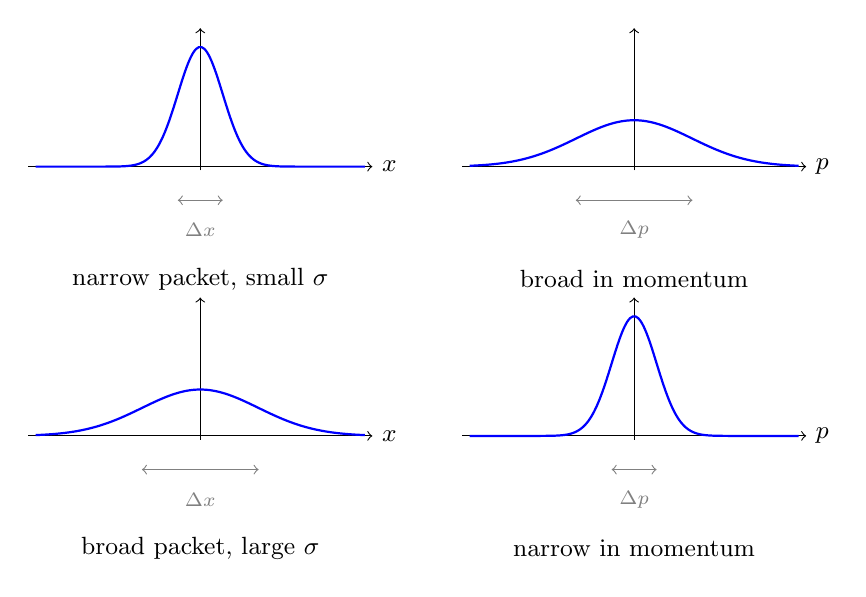
\begin{tikzpicture}[scale=0.95]
% Row 1: narrow in x, wide in p
\begin{scope}
\draw[->] (-2.3,0) -- (2.3,0) node[right] {\small $x$};
\draw[->] (0,-0.05) -- (0,1.85);
\draw[thick, color=blue, samples=120, smooth, domain=-2.2:2.2] plot (\x, {1.6*exp(-\x*\x/0.18)});
\draw[<->, gray] (-0.3,-0.45) -- (0.3,-0.45);
\node[gray] at (0,-0.85) {\scriptsize $\Delta x$};
\node at (0,-1.5) {\small narrow packet, small $\sigma$};
\end{scope}
\begin{scope}[shift={(5.8,0)}]
\draw[->] (-2.3,0) -- (2.3,0) node[right] {\small $p$};
\draw[->] (0,-0.05) -- (0,1.85);
\draw[thick, color=blue, samples=120, smooth, domain=-2.2:2.2] plot (\x, {0.62*exp(-\x*\x/1.2)});
\draw[<->, gray] (-0.78,-0.45) -- (0.78,-0.45);
\node[gray] at (0,-0.85) {\scriptsize $\Delta p$};
\node at (0,-1.5) {\small broad in momentum};
\end{scope}
% Row 2: wide in x, narrow in p
\begin{scope}[shift={(0,-3.6)}]
\draw[->] (-2.3,0) -- (2.3,0) node[right] {\small $x$};
\draw[->] (0,-0.05) -- (0,1.85);
\draw[thick, color=blue, samples=120, smooth, domain=-2.2:2.2] plot (\x, {0.62*exp(-\x*\x/1.2)});
\draw[<->, gray] (-0.78,-0.45) -- (0.78,-0.45);
\node[gray] at (0,-0.85) {\scriptsize $\Delta x$};
\node at (0,-1.5) {\small broad packet, large $\sigma$};
\end{scope}
\begin{scope}[shift={(5.8,-3.6)}]
\draw[->] (-2.3,0) -- (2.3,0) node[right] {\small $p$};
\draw[->] (0,-0.05) -- (0,1.85);
\draw[thick, color=blue, samples=120, smooth, domain=-2.2:2.2] plot (\x, {1.6*exp(-\x*\x/0.18)});
\draw[<->, gray] (-0.3,-0.45) -- (0.3,-0.45);
\node[gray] at (0,-0.85) {\scriptsize $\Delta p$};
\node at (0,-1.5) {\small narrow in momentum};
\end{scope}
\end{tikzpicture}
\end{center}

Squeezing the packet in position necessarily broadens it in momentum, and vice versa -- which, given that the two are Fourier transforms of each other, is a theorem about Fourier analysis quite as much as about physics. In the limits $\sigma \to 0$ and $\sigma \to \infty$ we approach the (non-normalisable) states $\ket{x}$ and $\ket{p}$ respectively, with one uncertainty going to zero and the other diverging.

\section{Time Evolution}

So far the formalism is entirely kinematic: it describes states at one instant. We now add dynamics, and in doing so we will meet a theme that runs through the rest of the course -- that a continuous symmetry is implemented by a family of unitary operators, and is `generated' by a Hermitian observable.

\subsection{The Evolution Operator}

\begin{axiom}[Time Evolution]
    The state of an isolated system evolves according to the \vocab{Schr\"odinger equation}
    $$
    i \hbar \frac{\dd}{\dd t} \ket{\psi(t)} = H \ket{\psi(t)},
    $$
    where the Hamiltonian $H$ is the observable corresponding to the energy of the system.
\end{axiom}

Since the equation is first order in $t$ and linear, the state at time $t$ is determined by the state at time $0$ by a linear operator:
$$
\ket{\psi(t)} = U(t) \ket{\psi(0)}.
$$
$U(t)$ is the \vocab{time evolution operator}. Substituting into the Schr\"odinger equation, and demanding it hold for all initial states, gives the operator equation
$$
i\hbar \frac{\dd U}{\dd t} = H U(t), \qquad U(0) = I,
$$
which for a time-independent $H$ has the solution
$$
U(t) = \exp\left(-\frac{i H t}{\hbar}\right),
$$
where the exponential is defined by the spectral decomposition (or, equivalently here, by its power series). The key property is the following.

\begin{proposition}
    $U(t)$ is unitary, and $U(s)U(t) = U(s+t)$, $U(t)^{-1} = U(-t)$.
\end{proposition}
\begin{proof}
    The group property is immediate from the exponential form (the exponents commute). For unitarity, note that $H^\dagger = H$ gives $U(t)^\dagger = \exp(+iHt/\hbar) = U(-t)$, so $U(t)^\dagger U(t) = U(0) = I$. Alternatively, and more instructively, one can prove it without solving anything: for any $\ket{\psi(t)}$ obeying the Schr\"odinger equation,
    $$
    \frac{\dd}{\dd t}\braket{\psi}{\psi} = \braket{\dot\psi}{\psi} + \braket{\psi}{\dot\psi} = \frac{i}{\hbar}\mel{\psi}{H^\dagger}{\psi} - \frac{i}{\hbar}\mel{\psi}{H}{\psi} = 0
    $$
    exactly because $H$ is Hermitian. So the norm -- total probability -- is conserved.
\end{proof}

This is the first instance of a pattern we will see repeatedly. A one-parameter family of unitaries $U(t) = e^{-iHt/\hbar}$ with $U(0) = I$ is determined by its derivative at the identity,
$$
H = i \hbar \left.\frac{\dd U}{\dd t}\right|_{t=0},
$$
and this derivative is Hermitian precisely because the $U(t)$ are unitary. We say $H$ \vocab{generates} time translations. In \S\ref{sec:symmetry} momentum will generate spatial translations and angular momentum will generate rotations, by exactly the same argument.

Solving the dynamics is now a matter of diagonalising $H$. If $H\ket{n} = E_n\ket{n}$ with $\{\ket{n}\}$ an orthonormal basis, then expanding $\ket{\psi(0)} = \sum_n a_n \ket{n}$,
$$
\ket{\psi(t)} = \sum_n a_n e^{-iE_n t/\hbar}\ket{n}, \qquad a_n = \braket{n}{\psi(0)}.
$$
Time evolution simply attaches a phase to each energy eigenstate. In particular a state which starts as an energy eigenstate stays one, acquiring only an overall phase -- these are the \vocab{stationary states}, physically unchanging.

\begin{remark}[Time-Dependent Hamiltonians]
    If $H = H(t)$, the formula $U(t) = \exp(-\frac{i}{\hbar}\int_0^t H(t')\dd t')$ is \emph{wrong} in general, because $H(t_1)$ and $H(t_2)$ need not commute. The correct expression is a time-ordered exponential, obtained by iterating the integral equation $U(t) = I - \frac{i}{\hbar}\int_0^t H(t')U(t')\dd t'$. We will construct the first two terms of this series when we do time-dependent perturbation theory in \S\ref{sec:tdpt}. Unitarity of $U(t)$, however, holds regardless, by the norm-conservation argument above.
\end{remark}

\subsection{The Heisenberg Picture}

There is a redundancy in the formalism: all physical predictions are matrix elements $\mel{\phi(t)}{A}{\psi(t)}$, and we can move the time dependence between the states and the operators at will. Writing the evolution out,
$$
\mel{\phi(t)}{A}{\psi(t)} = \mel{\phi(0)}{U(t)^\dagger A \, U(t)}{\psi(0)},
$$
we may either regard the states as evolving with $A$ fixed -- the \vocab{Schr\"odinger picture}, which is what we have been doing -- or regard the states as fixed and the operators as evolving.

\begin{definition}[Heisenberg Picture]
    In the \vocab{Heisenberg picture} the states are the fixed vectors $\ket{\psi}_H = \ket{\psi(0)}$, and observables carry the time dependence:
    $$
    A_H(t) = U(t)^\dagger A \, U(t).
    $$
\end{definition}

By construction the two pictures agree on every matrix element, hence on every physical prediction, and they agree at $t=0$. Note that $A_H(t)$ is Hermitian if $A$ is, that the transformation preserves all algebraic relations,
$$
(AB)_H = U^\dagger A B U = U^\dagger A U U^\dagger B U = A_H B_H, \qquad [A,B]_H = [A_H, B_H],
$$
and that $H_H = H$ when $H$ is time-independent (it commutes with $U$). Differentiating the definition gives the dynamical law.

\begin{theorem}[Heisenberg's Equation of Motion]
    For a time-independent Hamiltonian and a Schr\"odinger-picture operator $A$ which may itself depend explicitly on $t$,
    $$
    \frac{\dd A_H}{\dd t} = \frac{i}{\hbar}\left[ H, A_H \right] + \left( \frac{\partial A}{\partial t} \right)_{\!H}.
    $$
\end{theorem}
\begin{proof}
    Using $\dd U/\dd t = -\frac{i}{\hbar}HU$ and $\dd U^\dagger/\dd t = \frac{i}{\hbar}U^\dagger H$,
    $$
    \frac{\dd}{\dd t}\left( U^\dagger A U \right) = \frac{i}{\hbar}U^\dagger H A U - \frac{i}{\hbar} U^\dagger A H U + U^\dagger \frac{\partial A}{\partial t} U = \frac{i}{\hbar}U^\dagger[H,A]U + \left(\frac{\partial A}{\partial t}\right)_H,
    $$
    and $U^\dagger[H,A]U = [H_H, A_H] = [H,A_H]$. \qedhere
\end{proof}

This is a beautiful result, because it is \emph{formally identical to Hamilton's equations of classical mechanics}, with the Poisson bracket replaced by $\frac{1}{i\hbar}$ times the commutator:
$$
\frac{\dd f}{\dd t} = \{f, H\}_{\mathrm{PB}} + \frac{\partial f}{\partial t} \qquad \leadsto \qquad \frac{\dd A_H}{\dd t} = \frac{1}{i\hbar}[A_H, H] + \left(\frac{\partial A}{\partial t}\right)_H.
$$
Taking expectation values in any fixed state recovers, in the Schr\"odinger picture, \vocab{Ehrenfest's theorem}:
$$
\frac{\dd}{\dd t}\expval{A}_{\psi(t)} = \frac{i}{\hbar}\expval{[H,A]}_{\psi(t)} + \expval{\frac{\partial A}{\partial t}}_{\psi(t)}.
$$

\begin{corollary}[Conserved Quantities]
    If $A$ has no explicit time dependence and $[A, H] = 0$, then $A_H$ is constant, and $\expval{A}$ and indeed the whole probability distribution of $A$ are constant in time.
\end{corollary}

The last claim follows because the eigenprojectors of $A$ also commute with $H$, so $\mel{\psi(t)}{P_n}{\psi(t)} = \mel{\psi(0)}{U^\dagger P_n U}{\psi(0)} = \mel{\psi(0)}{P_n}{\psi(0)}$. Conservation laws in quantum mechanics are therefore exactly statements that observables commute with the Hamiltonian -- and, since the eigenvalues of $H$ label energies, they are also statements that the observable can be simultaneously diagonalised with the energy. This is the tight link between symmetry, conservation and degeneracy that \S\ref{sec:symmetry} makes systematic.

\begin{example}[The Free Particle]
    For $H = P^2/2m$ we have $[H,P] = 0$, so $P_H(t) = P$: momentum is conserved, as classically. For position, $[H, X] = \frac{1}{2m}[P^2, X] = \frac{1}{2m}\left(P[P,X] + [P,X]P\right) = -\frac{i\hbar}{m}P$, so
    $$
    \frac{\dd X_H}{\dd t} = \frac{i}{\hbar}\left(-\frac{i\hbar P}{m}\right) = \frac{P}{m}, \qquad \text{hence} \qquad X_H(t) = X + \frac{P t}{m}.
    $$
    This is exactly the classical solution, now as an operator identity. It has genuine content: for instance
    $$
    [X_H(t), X_H(0)] = \frac{t}{m}[P, X] = -\frac{i\hbar t}{m},
    $$
    so positions at different times are \emph{incompatible} observables, and we recover the spreading of a free wavepacket,
    $$
    (\Delta X)_t^2 = \expval{X_H(t)^2} - \expval{X_H(t)}^2 = (\Delta X)_0^2 + \frac{t}{m}\expval{XP + PX}_c + \frac{t^2}{m^2}(\Delta P)^2,
    $$
    where the middle term is the connected correlator $\expval{XP+PX} - 2\expval{X}\expval{P}$. For large $t$ the packet spreads linearly with rate $\Delta P/m$, which is just the classical statement that a spread of velocities produces a spread of positions.
\end{example}

\begin{remark}[Time-Energy Uncertainty]
    There is no time operator in quantum mechanics -- $t$ is a parameter, not an observable -- so `$\Delta E \Delta t \geq \hbar/2$' cannot be an instance of the generalised uncertainty principle. It can, however, be given a precise meaning. For any observable $A$ with no explicit time dependence, Ehrenfest plus the uncertainty relation give
    $$
    \Delta E \, \Delta A \geq \frac{1}{2}\abs{\expval{[H,A]}} = \frac{\hbar}{2}\abs{\frac{\dd \expval{A}}{\dd t}},
    $$
    so defining $\tau_A = \Delta A / \abs{\dd\expval{A}/\dd t}$ -- the time needed for $\expval{A}$ to shift by one standard deviation, i.e.\ the timescale on which the change is detectable -- we get $\Delta E \, \tau_A \geq \hbar/2$. A state of sharp energy is stationary and nothing ever happens in it; things can only change on a timescale set by the energy spread.
\end{remark}

\section{The Harmonic Oscillator}

Every quantum system that oscillates is, near equilibrium, a harmonic oscillator, and in IB we solved it by grinding through Hermite's equation. We now solve it again in three-quarters of a page, using nothing but the commutator $[X,P] = i\hbar$. This is not merely a labour-saving trick: the method -- find operators that step between eigenstates, then bound the spectrum below -- is exactly the method we will use for angular momentum, and the operators we build are the foundation of quantum field theory.

\subsection{Creation and Annihilation Operators}

The Hamiltonian is
$$
H = \frac{P^2}{2m} + \frac{1}{2}m\omega^2 X^2.
$$
If $X$ and $P$ were numbers we would factorise this as a product of $(\cdot + i \cdot)$ and $(\cdot - i\cdot)$. They are not, but let us try anyway.

\begin{definition}[Annihilation and Creation Operators]
    Set
    $$
    a = \sqrt{\frac{m\omega}{2\hbar}}\left( X + \frac{i P}{m\omega} \right), \qquad
    a^\dagger = \sqrt{\frac{m\omega}{2\hbar}}\left( X - \frac{i P}{m\omega} \right),
    $$
    the \vocab{annihilation} and \vocab{creation} operators. (The normalisation is chosen to make them dimensionless.)
\end{definition}

These are adjoints of one another, as the notation says, since $X$ and $P$ are Hermitian; they are not themselves Hermitian, and are the first non-Hermitian operators we have found a use for. Inverting,
$$
X = \sqrt{\frac{\hbar}{2m\omega}}\left(a + a^\dagger\right), \qquad P = -i\sqrt{\frac{m\hbar\omega}{2}}\left(a - a^\dagger\right),
$$
which we will use constantly -- almost every harmonic-oscillator computation in the rest of the course is done by substituting these and reading off the answer.

The single fact we need is:
$$
[a, a^\dagger] = \frac{m\omega}{2\hbar}\left( \left[X + \frac{iP}{m\omega}, X - \frac{iP}{m\omega}\right] \right) = \frac{m\omega}{2\hbar}\cdot\frac{-2i}{m\omega}[X,P] = \frac{m\omega}{2\hbar}\cdot\frac{-2i}{m\omega}\cdot i\hbar = 1.
$$
Now compute the product:
$$
a^\dagger a = \frac{m\omega}{2\hbar}\left( X^2 + \frac{P^2}{m^2\omega^2} + \frac{i}{m\omega}[X, P] \right) = \frac{H}{\hbar\omega} - \frac{1}{2}.
$$

\begin{definition}[Number Operator]
    $N = a^\dagger a$, so that $H = \hbar\omega\left(N + \frac{1}{2}\right)$.
\end{definition}

$N$ is Hermitian, and finding the spectrum of $H$ is now the same as finding the spectrum of $N$. The Leibniz rule and $[a,a^\dagger]=1$ give the two commutators that do all the work:
$$
[N, a] = [a^\dagger a, a] = [a^\dagger, a] a = -a, \qquad [N, a^\dagger] = a^\dagger [a, a^\dagger] = a^\dagger.
$$

\subsection{The Spectrum}

\begin{theorem}[Spectrum of the Harmonic Oscillator]
    The eigenvalues of $N$ are exactly $n = 0, 1, 2, \dots$, each non-degenerate, so
    $$
    E_n = \left(n + \frac{1}{2}\right)\hbar\omega, \qquad n \in \Z_{\geq 0}.
    $$
    Writing $\ket{n}$ for the normalised eigenstate of $N$ with eigenvalue $n$,
    $$
    a\ket{n} = \sqrt{n}\ket{n-1}, \qquad a^\dagger \ket{n} = \sqrt{n+1}\ket{n+1}, \qquad \ket{n} = \frac{(a^\dagger)^n}{\sqrt{n!}}\ket{0}.
    $$
\end{theorem}
\begin{proof}
    Suppose $N\ket{\nu} = \nu \ket{\nu}$ with $\ket{\nu}$ normalised. First,
    $$
    \nu = \mel{\nu}{a^\dagger a}{\nu} = \norm{a\ket{\nu}}^2 \geq 0,
    $$
    so all eigenvalues are non-negative, with $\nu = 0$ if and only if $a \ket{\nu} = 0$. Next, using $[N,a] = -a$,
    $$
    N \left( a \ket{\nu} \right) = \left( aN - a \right)\ket{\nu} = (\nu - 1) a\ket{\nu},
    $$
    so $a\ket{\nu}$ is either zero or an eigenvector with eigenvalue $\nu - 1$; similarly $N(a^\dagger \ket{\nu}) = (\nu+1)a^\dagger\ket{\nu}$, with $\norm{a^\dagger\ket{\nu}}^2 = \mel{\nu}{aa^\dagger}{\nu} = \nu + 1 > 0$, so $a^\dagger \ket{\nu}$ is never zero.

    Now suppose $\nu$ is not a non-negative integer. Then applying $a$ repeatedly produces eigenvectors with eigenvalues $\nu - 1, \nu - 2, \dots$, and none of them can ever be zero (a vector is zero only if its eigenvalue was $0$, which never occurs in this sequence). But eventually the eigenvalues become negative, contradicting $\nu \geq 0$. Hence $\nu = n \in \Z_{\geq 0}$, and the descending sequence terminates cleanly at $\ket{0}$ with $a\ket{0} = 0$.

    Conversely such states exist: $\ket{0}$ exists (we exhibit it in the next subsection), and $(a^\dagger)^n\ket{0}$ is a non-zero eigenvector with eigenvalue $n$. The normalisations follow from $\norm{a\ket{n}}^2 = n$ and $\norm{a^\dagger \ket{n}}^2 = n+1$, choosing phases so that both constants are positive; iterating $a^\dagger\ket{n} = \sqrt{n+1}\ket{n+1}$ gives $\ket{n} = (a^\dagger)^n\ket{0}/\sqrt{n!}$.

    Finally, non-degeneracy. In the position representation $a\ket{0} = 0$ reads
    $$
    \left( x + \frac{\hbar}{m\omega}\frac{\dd}{\dd x} \right)\psi_0(x) = 0,
    $$
    a first-order linear ODE with a one-dimensional solution space. So the ground state is unique, and since every $\ket{n}$ is obtained from it by $(a^\dagger)^n$ -- and conversely any eigenvector of eigenvalue $n$ is mapped by $a^n$ into the $\nu = 0$ eigenspace -- every level is non-degenerate.
\end{proof}

So the spectrum is an evenly spaced ladder, with $a^\dagger$ climbing it and $a$ descending it. It is worth drawing.

\begin{center}
\begin{tikzpicture}[scale=1.0]
\foreach \n/\lab/\en in {0/0/{\tfrac{1}{2}}, 1/1/{\tfrac{3}{2}}, 2/2/{\tfrac{5}{2}}, 3/3/{\tfrac{7}{2}}} {
  \draw[thick] (0,1.1*\n) -- (3.4,1.1*\n);
  \node[left] at (-0.15,1.1*\n) {$\ket{\lab}$};
  \node[right] at (3.6,1.1*\n) {$E_\lab = \en \hbar\omega$};
}
\draw[thick, dotted] (0,4.4) -- (3.4,4.4);
\node[left] at (-0.15,4.4) {$\vdots$};
% a-dagger arrows (up)
\foreach \n in {0,1,2,3} {
  \draw[->, thick, color=blue] (1.0,1.1*\n+0.09) -- (1.0,1.1*\n+1.01);
}
\node[left, color=blue] at (0.9,2.75) {$a^\dagger$};
% a arrows (down)
\foreach \n in {1,2,3,4} {
  \draw[->, thick, color=examplefg] (2.4,1.1*\n-0.09) -- (2.4,1.1*\n-1.01);
}
\node[right, color=examplefg] at (2.5,2.75) {$a$};
% annihilation at the bottom
\draw[->, thick, color=examplefg] (2.4,-0.09) -- (2.4,-0.8);
\node[right, color=examplefg] at (2.5,-0.55) {$a\ket{0} = 0$};
\end{tikzpicture}
\end{center}

The operators are named for what the picture shows: $a^\dagger$ creates a quantum of energy $\hbar\omega$ and $a$ annihilates one. The state $\ket{n}$ is naturally thought of not as `the $n$th excited state of one oscillator' but as `$n$ identical quanta', with $N$ counting them and $\ket{0}$ the \vocab{vacuum}. Applied to the modes of the electromagnetic field, those quanta are photons; this reinterpretation is the beginning of quantum field theory, and it is why this small piece of algebra is so important.

\subsection{Wavefunctions and Matrix Elements}

We can now recover the IB results with no differential equations beyond the first-order one above. Solving $\psi_0' = -(m\omega/\hbar)x\psi_0$ and normalising,
$$
\psi_0(x) = \braket{x}{0} = \left( \frac{m\omega}{\pi\hbar} \right)^{1/4} \exp\left( -\frac{m\omega x^2}{2\hbar} \right),
$$
a Gaussian -- and, by \S\ref{sec:wavepackets}, a minimum uncertainty state. The excited states follow by applying
$$
a^\dagger = \sqrt{\frac{m\omega}{2\hbar}}\left( x - \frac{\hbar}{m\omega}\frac{\dd}{\dd x} \right)
$$
repeatedly, which manufactures a Hermite polynomial times the Gaussian at each step; for instance
$$
\psi_1(x) \propto \left(x - \frac{\hbar}{m\omega}\frac{\dd}{\dd x}\right) e^{-m\omega x^2/2\hbar} = 2x \, e^{-m\omega x^2/2\hbar},
$$
matching $H_1(\xi) = 2\xi$. Orthonormality of the $\ket{n}$ is automatic (eigenvectors of a Hermitian operator with distinct eigenvalues), which saves proving any Hermite polynomial identities at all.

More useful in practice are matrix elements. From $X = \sqrt{\hbar/2m\omega}(a + a^\dagger)$,
$$
\mel{m}{X}{n} = \sqrt{\frac{\hbar}{2m\omega}}\left( \sqrt{n}\,\delta_{m,n-1} + \sqrt{n+1}\,\delta_{m,n+1} \right),
$$
so $X$ connects only neighbouring levels -- a selection rule which we will use in perturbation theory. Similarly
$$
\mel{m}{P}{n} = i\sqrt{\frac{m\hbar\omega}{2}}\left( \sqrt{n+1}\,\delta_{m,n+1} - \sqrt{n}\,\delta_{m,n-1} \right).
$$

\begin{example}[Uncertainties in the Level $\ket{n}$]
    Since $\mel{n}{X}{n} = \mel{n}{P}{n} = 0$, we need only the squares. Expanding,
    $$
    X^2 = \frac{\hbar}{2m\omega}\left( a^2 + (a^\dagger)^2 + a a^\dagger + a^\dagger a \right),
    $$
    and $\mel{n}{a^2}{n} = \mel{n}{(a^\dagger)^2}{n} = 0$ (they change the level by two), while $a^\dagger a = N$ and $aa^\dagger = N+1$. Hence
    $$
    \expval{X^2}_n = \frac{\hbar}{2m\omega}(2n+1) = \frac{\hbar}{m\omega}\left(n + \frac{1}{2}\right),
    $$
    and identically $\expval{P^2}_n = m\hbar\omega\left(n + \frac12\right)$. Therefore
    $$
    \Delta X \, \Delta P = \left(n + \frac{1}{2}\right)\hbar,
    $$
    saturating the uncertainty bound only in the ground state, as expected. Note also that $\expval{P^2/2m}_n = \expval{\frac12 m\omega^2X^2}_n = \frac12 E_n$: kinetic and potential energy contribute equally, which is the quantum virial theorem for a quadratic potential.
\end{example}

\begin{example}[The Oscillator in the Heisenberg Picture]
    The Heisenberg equation for $a$ is especially clean. Since $[H, a] = \hbar\omega[N,a] = -\hbar\omega a$,
    $$
    \frac{\dd a_H}{\dd t} = \frac{i}{\hbar}[H, a_H] = -i\omega a_H \qquad \Longrightarrow \qquad a_H(t) = a \, e^{-i\omega t},
    $$
    and taking adjoints $a_H^\dagger(t) = a^\dagger e^{i\omega t}$. Substituting into $X = \sqrt{\hbar/2m\omega}(a + a^\dagger)$ gives
    $$
    X_H(t) = X\cos\omega t + \frac{P}{m\omega}\sin\omega t, \qquad P_H(t) = P \cos\omega t - m\omega X \sin\omega t,
    $$
    which is precisely the classical solution, holding now as an operator identity. This is Ehrenfest's theorem in its most satisfying form: for a quadratic Hamiltonian the expectation values follow the classical trajectory \emph{exactly}, for every state.
\end{example}

\begin{remark}[Coherent States]
    Since $a$ is not Hermitian its eigenvalues need not be real, and in fact $a$ has an eigenstate for \emph{every} complex number $\alpha$:
    $$
    \ket{\alpha} = e^{-\abs{\alpha}^2/2}\sum_{n \geq 0}\frac{\alpha^n}{\sqrt{n!}}\ket{n}, \qquad a \ket{\alpha} = \alpha \ket{\alpha},
    $$
    as one checks by applying $a$ term by term. These \vocab{coherent states} are minimum-uncertainty Gaussians displaced from the origin, and under time evolution $\ket{\alpha} \mapsto \ket{\alpha e^{-i\omega t}}$ -- a wavepacket that oscillates back and forth without ever spreading, tracing out the classical motion. They are the closest thing quantum mechanics has to a classical oscillator, and are the states produced by a laser.
\end{remark}

\begin{example}[The Three-Dimensional Isotropic Oscillator]
    For $H = \frac{\vv{P}^2}{2m} + \frac12 m\omega^2 \vv{X}^2$ the three directions decouple: with $a_i$ built from $X_i, P_i$ we have $[a_i, a_j^\dagger] = \delta_{ij}$ and
    $$
    H = \hbar\omega\left( N_1 + N_2 + N_3 + \frac{3}{2} \right),
    $$
    so $E = (n + \frac32)\hbar\omega$ with $n = n_1+n_2+n_3$. The degeneracy of the level $n$ is the number of ways to write $n$ as an ordered sum of three non-negative integers, namely $\binom{n+2}{2} = \frac12(n+1)(n+2)$: so $1, 3, 6, 10, \dots$. Some of this is explained by rotational symmetry (\S\ref{sec:symmetry}), but not all of it -- the isotropic oscillator, like the hydrogen atom, has a `hidden' symmetry larger than rotations.
\end{example}

\section{Angular Momentum}\label{sec:angmom}

In IB we found that the orbital angular momentum operators $L_i = \epsilon_{ijk}X_jP_k$ satisfy
$$
[L_i, L_j] = i\hbar\,\epsilon_{ijk}L_k,
$$
and that solving the associated differential equations gives the spherical harmonics, with $\ell$ a non-negative integer. We now run the harmonic-oscillator strategy on this problem: forget where the operators came from, keep only the commutation relations, and see what the algebra forces. The answer will turn out to be strictly richer than what the differential equations gave us -- half-integer values appear, and they are realised in nature as \emph{spin}, an angular momentum with no classical or orbital counterpart at all.

\subsection{The Algebra}

\begin{definition}[Angular Momentum]
    An \vocab{angular momentum} is a triple of Hermitian operators $J_1, J_2, J_3$ on $\mathcal{H}$ satisfying
    $$
    [J_i, J_j] = i \hbar \, \epsilon_{ijk} J_k.
    $$
    We write $J^2 = J_1^2 + J_2^2 + J_3^2$, and usually $J_z$ for $J_3$.
\end{definition}

Written out, the relations are $[J_1,J_2] = i\hbar J_3$ and its cyclic images. The first thing to check is that although no two components are compatible, the total is compatible with each one.

\begin{proposition}
    $[J^2, J_i] = 0$ for each $i$.
\end{proposition}
\begin{proof}
    Take $i = 3$; the rest follow by relabelling. Using $[A, B^2] = B[A,B] + [A,B]B$,
    $$
    [J_1^2, J_3] = J_1[J_1,J_3] + [J_1,J_3]J_1 = -i\hbar(J_1 J_2 + J_2 J_1),
    $$
    $$
    [J_2^2, J_3] = J_2[J_2,J_3] + [J_2,J_3]J_2 = i\hbar(J_2 J_1 + J_1 J_2),
    $$
    and $[J_3^2, J_3] = 0$. The two non-zero pieces cancel.
\end{proof}

So $\{J^2, J_z\}$ is a commuting pair, and we look for their simultaneous eigenstates. This is the best we can do -- the length of the angular momentum vector and one of its components -- and the choice of $z$ is pure convention.

\begin{definition}[Ladder Operators]
    $J_\pm = J_1 \pm i J_2$, so that $J_\pm^\dagger = J_\mp$.
\end{definition}

The relations we need are all immediate:
$$
[J_z, J_\pm] = \pm \hbar J_\pm, \qquad [J_+, J_-] = 2\hbar J_z, \qquad [J^2, J_\pm] = 0,
$$
and, expanding the products and using $[J_1,J_2] = i\hbar J_3$,
$$
J_-J_+ = (J_1-iJ_2)(J_1+iJ_2) = J_1^2 + J_2^2 + i[J_1,J_2] = J^2 - J_z^2 - \hbar J_z,
$$
and, changing the sign of $i$ throughout, $J_+J_- = J^2 - J_z^2 + \hbar J_z$. The first of these commutators, $[J_z, J_\pm] = \pm\hbar J_\pm$, is exactly the relation $[N, a^\dagger] = a^\dagger$ that made the oscillator work, and it does the same job here.

\subsection{The Spectrum}

\begin{theorem}[Spectrum of Angular Momentum]
    Let $\ket{\psi}$ be a simultaneous eigenstate of $J^2$ and $J_z$. Then the eigenvalues take the form
    $$
    J^2 \ket{j\,m} = \hbar^2 j(j+1)\ket{j\,m}, \qquad J_z \ket{j\, m} = \hbar m \ket{j\,m},
    $$
    where
    $$
    j \in \left\{ 0, \tfrac12, 1, \tfrac32, 2, \dots \right\}, \qquad m \in \{-j, -j+1, \dots, j-1, j\}.
    $$
    Moreover, with a suitable choice of phases,
    $$
    J_\pm \ket{j\,m} = \hbar\sqrt{j(j+1) - m(m\pm1)}\,\ket{j\, m\pm 1}.
    $$
\end{theorem}
\begin{proof}
    Write the eigenvalues as $J^2\ket{\psi} = \hbar^2\lambda\ket{\psi}$ and $J_z\ket{\psi} = \hbar m \ket{\psi}$ with $\ket{\psi}$ normalised.

    \emph{Step 1: a bound.} Since $J^2 - J_z^2 = J_1^2 + J_2^2$ and each $J_i$ is Hermitian,
    $$
    \hbar^2(\lambda - m^2) = \mel{\psi}{J_1^2 + J_2^2}{\psi} = \norm{J_1\ket{\psi}}^2 + \norm{J_2\ket{\psi}}^2 \geq 0,
    $$
    so $\lambda \geq m^2$: for fixed $\lambda$ the possible $m$ are bounded above and below.

    \emph{Step 2: the ladder.} Since $[J^2, J_\pm] = 0$ and $[J_z, J_\pm] = \pm\hbar J_\pm$,
    $$
    J^2 \left( J_\pm \ket{\psi} \right) = \hbar^2 \lambda \left( J_\pm\ket{\psi}\right), \qquad J_z \left(J_\pm\ket{\psi}\right) = \hbar(m\pm1)\left(J_\pm\ket{\psi}\right),
    $$
    so $J_\pm$ moves $m$ by one while preserving $\lambda$ -- unless it gives zero. And its norm is computable:
    $$
    \norm{J_\pm \ket{\psi}}^2 = \mel{\psi}{J_\mp J_\pm}{\psi} = \mel{\psi}{J^2 - J_z^2 \mp \hbar J_z}{\psi} = \hbar^2 \left( \lambda - m(m\pm1) \right).
    $$

    \emph{Step 3: termination.} By Step 1 the sequence $\ket\psi, J_+\ket\psi, J_+^2\ket\psi, \dots$ cannot continue for ever, so there is a top state with $J_z$ eigenvalue $\hbar j$ (say) killed by $J_+$; by Step 2, $\lambda = j(j+1)$. Likewise there is a bottom state with eigenvalue $\hbar m_{\min}$ killed by $J_-$, giving $\lambda = m_{\min}(m_{\min}-1)$. Setting the two equal,
    $$
    j(j+1) = m_{\min}(m_{\min}-1) \quad \Longrightarrow \quad m_{\min} = -j
    $$
    (the other root, $m_{\min} = j+1$, is impossible since $m_{\min}\leq j$).

    \emph{Step 4: quantisation.} The bottom state is reached from the top by applying $J_-$ some non-negative integer number of times, so $j - (-j) = 2j \in \Z_{\geq0}$: that is, $j$ is a non-negative integer or half-integer, and $m$ runs over $-j, -j+1, \dots, j$ in unit steps, giving $2j+1$ values. The normalisation constants come from Step 2, choosing all phases positive.
\end{proof}

Compare this with the IB derivation. There, integrality of $\ell$ came from demanding that $e^{im\phi}$ be single-valued on the sphere; here, quantisation comes from the algebra alone, and it permits half-integers. Both answers are correct: half-integer $j$ cannot occur for \emph{orbital} angular momentum (\S\ref{sec:orbital}), but nothing forbids it in general, and electrons, protons and neutrons all have $j = \frac12$.

\begin{center}
\begin{tikzpicture}[scale=1.0]
% ladder for j = 2
\foreach \m/\lab/\jz in {-2/{-2}/{-2\hbar}, -1/{-1}/{-\hbar}, 0/{0}/{0}, 1/{1}/{\hbar}, 2/{2}/{2\hbar}} {
  \draw[thick] (0,1.0*\m) -- (2.6,1.0*\m);
  \node[left] at (-0.15,1.0*\m) {$\ket{j\,\lab}$};
  \node[right] at (2.8,1.0*\m) {\small $J_z = \jz$};
}
\foreach \m in {-2,-1,0,1} {
  \draw[->, thick, color=blue] (0.75,1.0*\m+0.08) -- (0.75,1.0*\m+0.92);
  \draw[->, thick, color=examplefg] (1.85,1.0*\m+0.92) -- (1.85,1.0*\m+0.08);
}
\node[left, color=blue] at (0.66,1.5) {$J_+$};
\node[right, color=examplefg] at (1.94,1.5) {$J_-$};
% annihilation at the ends
\draw[->, thick, color=blue] (0.75,2.08) -- (0.75,2.75);
\node[right, color=blue] at (0.85,2.5) {\small $J_+\ket{j\,j} = 0$};
\draw[->, thick, color=examplefg] (1.85,-2.08) -- (1.85,-2.75);
\node[right, color=examplefg] at (1.95,-2.5) {\small $J_-\ket{j\,{-j}} = 0$};
\node at (1.3,-3.6) {\small the multiplet $j = 2$: five states, all with $J^2 = 6\hbar^2$};
\end{tikzpicture}
\end{center}

For each allowed $j$ the $2j+1$ states $\ket{j\,m}$ form a \vocab{multiplet}, closed under the action of all three $J_i$ (since $J_1, J_2$ are combinations of $J_\pm$). In the language of Representation Theory, a multiplet is an irreducible representation of the Lie algebra $\mathfrak{su}(2)$, and we have just classified them all. Nothing in the argument says which $j$ actually occur in a given physical system, or how many times -- that depends on the system.

\subsection{Matrix Representations and Spin}

Within a single multiplet the operators are finite matrices, which we can write down explicitly.

\begin{example}[$j = 0$]
    A single state $\ket{0\,0}$ with $J_i = 0$: no angular momentum at all.
\end{example}

\begin{example}[$j = \tfrac12$]
    Two states, $\ket{\tfrac12\,\tfrac12} =: \ket{\uparrow}$ and $\ket{\tfrac12\,{-\tfrac12}} =: \ket{\downarrow}$, spanning $\C^2$. From the theorem, $J_z = \frac{\hbar}{2}\mathrm{diag}(1,-1)$, and
    $$
    J_+\ket{\downarrow} = \hbar\ket{\uparrow}, \quad J_+\ket{\uparrow} = 0, \quad J_-\ket{\uparrow} = \hbar\ket{\downarrow}, \quad J_-\ket{\downarrow} = 0,
    $$
    so in the basis $(\ket\uparrow, \ket\downarrow)$,
    $$
    J_+ = \hbar\begin{pmatrix}0&1\\0&0\end{pmatrix}, \quad J_- = \hbar\begin{pmatrix}0&0\\1&0\end{pmatrix}, \quad \text{hence} \quad J_1 = \frac{J_++J_-}{2}, \; J_2 = \frac{J_+-J_-}{2i}.
    $$
    Writing $\vv{S} = \frac{\hbar}{2}\vv{\sigma}$ (the traditional notation for spin), this gives the \vocab{Pauli matrices}
    $$
    \sigma_1 = \begin{pmatrix}0&1\\1&0\end{pmatrix}, \qquad
    \sigma_2 = \begin{pmatrix}0&-i\\i&0\end{pmatrix}, \qquad
    \sigma_3 = \begin{pmatrix}1&0\\0&-1\end{pmatrix}.
    $$
\end{example}

\begin{example}[$j = 1$]
    Three states; in the basis $\ket{1\,1}, \ket{1\,0}, \ket{1\,{-1}}$, the coefficients $\sqrt{j(j+1)-m(m\pm1)}$ are all $\sqrt2$, so
    $$
    J_z = \hbar\begin{pmatrix}1&0&0\\0&0&0\\0&0&-1\end{pmatrix}, \quad
    J_+ = \sqrt2 \hbar\begin{pmatrix}0&1&0\\0&0&1\\0&0&0\end{pmatrix}, \quad
    J_1 = \frac{\hbar}{\sqrt2}\begin{pmatrix}0&1&0\\1&0&1\\0&1&0\end{pmatrix}.
    $$
    One can check $J^2 = 2\hbar^2 I$, as it must be.
\end{example}

The Pauli matrices deserve their own list of properties, since spin-$\frac12$ is by far the most important case.

\begin{proposition}[Pauli Algebra]
    The Pauli matrices are Hermitian and traceless, with $\sigma_i^2 = I$, and
    $$
    \sigma_i \sigma_j = \delta_{ij} I + i \epsilon_{ijk}\sigma_k.
    $$
    Consequently $[\sigma_i,\sigma_j] = 2i\epsilon_{ijk}\sigma_k$ and $\{\sigma_i,\sigma_j\} = 2\delta_{ij}I$, and for any unit vector $\vv{n}$,
    $$
    (\vv{n}\cdot\vv{\sigma})^2 = I, \qquad \exp\left( -\frac{i\theta}{2}\,\vv{n}\cdot\vv{\sigma} \right) = \cos\frac{\theta}{2}\, I - i \sin\frac{\theta}{2}\, \vv{n}\cdot\vv{\sigma}.
    $$
\end{proposition}
\begin{proof}
    The product rule is verified by multiplying the matrices out (or by noting that the symmetric part must be $\delta_{ij}I$ since $\sigma_i^2 = I$, and the antisymmetric part is $\frac12[\sigma_i,\sigma_j]$, which is the angular momentum relation). Then
    $$
    (\vv{n}\cdot\vv{\sigma})^2 = n_in_j\sigma_i\sigma_j = n_in_j\delta_{ij}I + i\epsilon_{ijk}n_in_j\sigma_k = \abs{\vv{n}}^2 I = I,
    $$
    the $\epsilon$ term dying by symmetry. The exponential then follows by splitting the power series into even and odd parts, exactly as for $e^{i\theta}$.
\end{proof}

Since $(\vv n \cdot \vv \sigma)^2 = I$, the operator $\vv{n}\cdot\vv{S} = \frac{\hbar}{2}\vv n \cdot \vv\sigma$ has eigenvalues $\pm\frac\hbar2$ for \emph{every} direction $\vv n$: a spin-$\frac12$ measurement along any axis gives one of two answers. Writing $\vv{n} = (\sin\theta\cos\phi, \sin\theta\sin\phi,\cos\theta)$, one finds the eigenstates
$$
\ket{\vv n \,\uparrow} = \cos\frac\theta2 \ket\uparrow + e^{i\phi}\sin\frac\theta2\ket\downarrow, \qquad
\ket{\vv n \,\downarrow} = -e^{-i\phi}\sin\frac\theta2 \ket\uparrow + \cos\frac\theta2\ket\downarrow.
$$
This is a bijection (up to phase) between unit vectors in $\R^3$ and states of a qubit, and gives the standard picture of the spin-$\frac12$ state space as a sphere.

\begin{center}
\begin{tikzpicture}[scale=1.8]
% sphere
\draw[thick] (0,0) circle (1);
\draw[dashed, gray] (-1,0) arc (180:360:1 and 0.3);
\draw[gray] (1,0) arc (0:180:1 and 0.3);
% axes
\draw[->] (0,-1.25) -- (0,1.3) node[above] {\small $z$};
\draw[->] (0,0) -- (1.32,0) node[right] {\small $y$};
\draw[->] (0,0) -- (-0.78,-0.6) node[below left] {\small $x$};
% state vector and its equatorial projection
\draw[->, very thick, color=blue] (0,0) -- (0.60,0.64);
\node[color=blue] at (0.72,0.76) {\small $\vv{n}$};
\draw[dashed, gray] (0.60,0.64) -- (0.60,0.19);
\draw[dashed, gray] (0,0) -- (0.60,0.19);
% angle theta
\draw[color=examplefg] (0,0.45) arc (90:46.8:0.45);
\node[color=examplefg] at (0.17,0.55) {\scriptsize $\theta$};
% angle phi in the equatorial plane
\draw[color=examplefg] (-0.30,-0.23) arc (217:17.5:0.31 and 0.10);
\node[color=examplefg] at (0.10,-0.20) {\scriptsize $\phi$};
% labels
\node[above right] at (0.04,1.0) {\small $\ket{\uparrow}$};
\node[below right] at (0.04,-1.0) {\small $\ket{\downarrow}$};
\fill (0,1) circle (0.022);
\fill (0,-1) circle (0.022);
\end{tikzpicture}
\end{center}

This is the \vocab{Bloch sphere}. Antipodal points are orthogonal states (note $\theta \mapsto \pi - \theta$, $\phi \mapsto \phi+\pi$ sends $\ket{\vv n \uparrow}$ to $\ket{\vv n \downarrow}$ up to phase), so the angle on the sphere is \emph{twice} the angle in Hilbert space -- another manifestation of the factor of $\frac12$ that pervades spin-$\frac12$.

\begin{example}[Measuring Spin in a Rotated Basis]
    Prepare a particle in $\ket\uparrow$ and measure $\vv n \cdot \vv S$. The probability of $+\frac\hbar2$ is
    $$
    \abs{\braket{\vv n \uparrow}{\uparrow}}^2 = \cos^2\frac\theta2 = \frac{1 + \cos\theta}{2},
    $$
    and of $-\frac\hbar2$ is $\sin^2\frac\theta2$. So $\expval{\vv n \cdot \vv S}_\uparrow = \frac\hbar2\cos\theta$: the expectation behaves like the projection of a classical vector of length $\frac\hbar2$ onto $\vv n$, even though every individual measurement returns $\pm\frac\hbar2$. For $\theta = \pi/2$ the two outcomes are equally likely -- a state with definite $S_z$ is maximally uncertain in $S_x$.
\end{example}

\subsection{The Stern--Gerlach Experiment}

Spin is not a mathematical curiosity: it was forced on physics by experiment. A neutral particle with spin has a magnetic moment proportional to it,
$$
\vv{\mu} = \gamma \vv{S},
$$
with $\gamma$ the \vocab{gyromagnetic ratio}, and in a magnetic field it acquires an energy $H = -\vv\mu\cdot\vv B$. In a field with a gradient the particle also feels a force $\nabla(\vv\mu\cdot\vv B)$, so a beam passing through an inhomogeneous field is deflected by an amount proportional to $\mu_z$ -- which is a direct measurement of $S_z$. Classically, an unpolarised beam has $\mu_z$ uniformly distributed and one expects a continuous smear on the screen. What Stern and Gerlach (1922) saw with silver atoms was two discrete spots.

\begin{center}
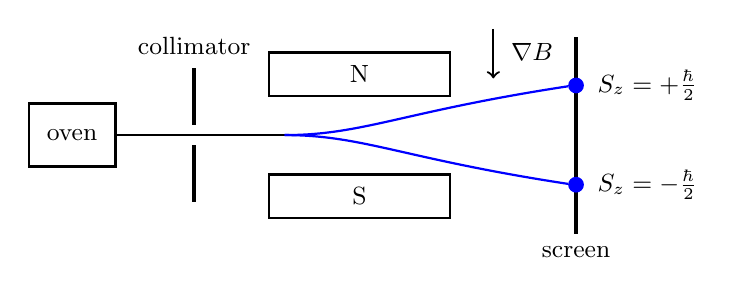
\begin{tikzpicture}[scale=1.0]
% source
\draw[thick] (-0.75,-0.4) rectangle (0.35,0.4);
\node at (-0.2,0) {\small oven};
\draw[thick] (0.35,0) -- (1.35,0);
% collimator
\draw[very thick] (1.35,0.13) -- (1.35,0.85);
\draw[very thick] (1.35,-0.13) -- (1.35,-0.85);
\node[above] at (1.35,0.9) {\small collimator};
% magnet poles
\draw[thick] (2.3,0.5) rectangle (4.6,1.05);
\node at (3.45,0.775) {\small N};
\draw[thick] (2.3,-0.5) rectangle (4.6,-1.05);
\node at (3.45,-0.775) {\small S};
\draw[->, thick] (5.15,1.35) -- (5.15,0.72);
\node[right] at (5.25,1.05) {\small $\nabla B$};
% beam
\draw[thick] (1.35,0) -- (2.5,0);
\draw[thick, color=blue] (2.5,0) .. controls (3.5,0) and (4.0,0.3) .. (6.1,0.62);
\draw[thick, color=blue] (2.5,0) .. controls (3.5,0) and (4.0,-0.3) .. (6.1,-0.62);
% screen
\draw[very thick] (6.2,-1.25) -- (6.2,1.25);
\fill[color=blue] (6.2,0.63) circle (0.1);
\fill[color=blue] (6.2,-0.63) circle (0.1);
\node[right] at (6.35,0.63) {\small $S_z = +\tfrac{\hbar}{2}$};
\node[right] at (6.35,-0.63) {\small $S_z = -\tfrac{\hbar}{2}$};
\node[below] at (6.2,-1.3) {\small screen};
\end{tikzpicture}
\end{center}

Two spots means two values of $S_z$, i.e.\ $2j+1 = 2$, i.e.\ $j = \frac12$ -- a value impossible for orbital angular momentum. The apparatus is also the cleanest illustration of the measurement postulate: block the lower beam, and the surviving atoms are all in $\ket\uparrow$; pass them through a second identical magnet and they all go up, but pass them through a magnet oriented along $x$ and they split $50$--$50$, in agreement with the example above. Recombining the two beams coherently, on the other hand, restores the original state entirely -- so long as no measurement records which path was taken.

\begin{example}[Larmor Precession]
    Put a spin in a uniform field $\vv B = B\vv{e}_3$. Then $H = -\gamma B S_z$, and using $[S_3,S_1] = i\hbar S_2$, $[S_3,S_2] = -i\hbar S_1$, the Heisenberg equations give
    $$
    \frac{\dd S_1}{\dd t} = -\gamma B\,\frac{i}{\hbar}[S_3, S_1] = \omega_L S_2, \qquad \frac{\dd S_2}{\dd t} = -\omega_L S_1, \qquad \frac{\dd S_3}{\dd t} = 0,
    $$
    where $\omega_L = \gamma B$. So $\expval{\vv S}$ precesses about the field at the \vocab{Larmor frequency} $\omega_L$, exactly like a classical gyroscope. In the Schr\"odinger picture the same statement is that $\ket\uparrow$ and $\ket\downarrow$ acquire phases $e^{\pm i\omega_L t/2}$, so a state initially along $\vv{e}_1$ becomes
    $$
    \frac{1}{\sqrt2}\left( e^{i\omega_L t/2}\ket\uparrow + e^{-i\omega_L t /2}\ket\downarrow \right),
    $$
    which is the spin pointing along $(\cos\omega_L t, -\sin\omega_L t, 0)$. Note that after a time $2\pi/\omega_L$ the \emph{spin direction} has returned but the \emph{state vector} has acquired a factor of $-1$; only after $4\pi$ of rotation does the state itself return.
\end{example}

\subsection{Orbital Angular Momentum}\label{sec:orbital}

Return now to $\vv L = \vv X \times \vv P$. One checks (as in IB, using $[X_i,P_j]=i\hbar\delta_{ij}$) that this satisfies the angular momentum algebra, so all of the above applies with $j = \ell$. The question is which $\ell$ occur.

In spherical polar coordinates $L_z = -i\hbar\,\partial_\phi$, and a slightly longer computation gives
$$
L_\pm = \hbar e^{\pm i \phi}\left( \pm \frac{\partial}{\partial\theta} + i \cot\theta \frac{\partial}{\partial\phi} \right).
$$
An eigenfunction of $L_z$ with eigenvalue $\hbar m$ has $\phi$-dependence $e^{im\phi}$, and single-valuedness on the sphere forces $m \in \Z$; hence $\ell \in \Z_{\geq0}$. \emph{Half-integer values are excluded for orbital angular momentum, but only by this topological input, which has no analogue for an intrinsic degree of freedom.} That is the precise sense in which spin is `not orbital'.

The ladder operators give a pleasant way to construct the spherical harmonics without touching Legendre's equation. The top state of the multiplet satisfies $L_+Y_{\ell\ell} = 0$, i.e.
$$
\left( \frac{\partial}{\partial\theta} - \ell\cot\theta \right) f(\theta) = 0 \quad \text{for } Y_{\ell\ell} = f(\theta)e^{i\ell\phi},
$$
whose solution is $f \propto \sin^\ell\theta$. So
$$
Y_{\ell\ell}(\theta,\phi) \propto \sin^\ell\theta \; e^{i\ell\phi},
$$
and every other $Y_{\ell m}$ follows by applying $L_-$ repeatedly, with the normalisations supplied by the theorem. For $\ell=1$ this gives $Y_{11}\propto \sin\theta e^{i\phi}$, then $L_-$ produces $Y_{10}\propto\cos\theta$ and $Y_{1,-1}\propto \sin\theta e^{-i\phi}$, matching IB.

\begin{remark}
    Notice how much less work this is than the differential equation route, and how much more it explains. The mysterious constraint $\abs{m}\leq\ell$ and the eigenvalue $\hbar^2\ell(\ell+1)$ (rather than $\hbar^2\ell^2$) are now consequences of the commutation relations, and the same algebra will hand us the whole theory of spin and of adding angular momenta.
\end{remark}

For a particle with spin moving in space, the total angular momentum is
$$
\vv{J} = \vv{L} + \vv{S},
$$
where $\vv L$ acts on the spatial factor of $\mathcal{H} = L^2(\R^3)\otimes\C^2$ and $\vv S$ on the spin factor. Since they act on different factors they commute, and one checks immediately that $\vv J$ satisfies the angular momentum algebra. Understanding the multiplet structure of such a sum is the subject of the next section.

\section{Composite Systems and Addition of Angular Momentum}

\subsection{Tensor Products}\label{sec:tensor}

If a system is built from two subsystems -- two particles, or the position and spin of one particle -- how do their Hilbert spaces combine? The answer is not a direct sum but a tensor product, and this innocuous-looking choice is the source of essentially everything strange about quantum mechanics.

\begin{definition}[Tensor Product]
    Let $\mathcal{H}_1, \mathcal{H}_2$ be Hilbert spaces with orthonormal bases $\{\ket{i}_1\}$, $\{\ket{a}_2\}$. Their \vocab{tensor product} $\mathcal{H}_1 \otimes \mathcal{H}_2$ is the Hilbert space with orthonormal basis $\{\ket{i}_1 \otimes \ket{a}_2\}$, and inner product determined by
    $$
    \left( \bra{\phi}_1\otimes\bra{\chi}_2 \right)\left( \ket{\psi}_1\otimes\ket{\omega}_2 \right) = \braket{\phi}{\psi}_1 \braket{\chi}{\omega}_2.
    $$
    The map $(\ket\psi_1, \ket\omega_2) \mapsto \ket\psi_1\otimes\ket\omega_2$ is bilinear.
\end{definition}

\begin{axiom}[Composite Systems]
    The state space of a system composed of two subsystems with state spaces $\mathcal{H}_1$ and $\mathcal{H}_2$ is $\mathcal{H}_1 \otimes \mathcal{H}_2$.
\end{axiom}

In particular $\dim(\mathcal{H}_1\otimes\mathcal{H}_2) = \dim\mathcal{H}_1 \cdot \dim\mathcal{H}_2$ -- dimensions multiply, they do not add. We will freely abbreviate $\ket\psi\otimes\ket\omega$ as $\ket\psi\ket\omega$ or $\ket{\psi\,\omega}$ when no confusion can arise. An operator $A$ on $\mathcal{H}_1$ acts on the product as $A \otimes I$, and
$$
(A\otimes B)(\ket\psi\otimes\ket\omega) = A\ket\psi\otimes B\ket\omega, \qquad (A\otimes B)(C \otimes D) = AC \otimes BD.
$$
Operators belonging to different factors always commute: $[A\otimes I, I \otimes B] = 0$. This is the formal statement that measurements on subsystem $1$ are compatible with measurements on subsystem $2$.

\begin{example}[Two Spins]
    For two spin-$\frac12$ particles, $\mathcal{H} = \C^2\otimes\C^2$ is four-dimensional with basis
    $$
    \ket{\uparrow\uparrow}, \quad \ket{\uparrow\downarrow}, \quad \ket{\downarrow\uparrow}, \quad \ket{\downarrow\downarrow}.
    $$
    A single spin-$\frac12$ particle in three dimensions has $\mathcal{H} = L^2(\R^3)\otimes\C^2$; a general state is $\ket\Psi = \ket{\psi_\uparrow}\otimes\ket\uparrow + \ket{\psi_\downarrow}\otimes\ket\downarrow$, conveniently written as a two-component \vocab{spinor} wavefunction
    $$
    \Psi(\vv x) = \begin{pmatrix} \psi_\uparrow(\vv x) \\ \psi_\downarrow(\vv x) \end{pmatrix},
    $$
    with $\abs{\psi_\uparrow(\vv x)}^2$ the probability density for finding the particle at $\vv x$ with spin up.
\end{example}

\begin{definition}[Entanglement]
    A state of $\mathcal{H}_1\otimes\mathcal{H}_2$ is a \vocab{product state} if it can be written as $\ket\psi\otimes\ket\omega$, and is \vocab{entangled} otherwise.
\end{definition}

Most states are entangled: a general state $\sum_{i,a}c_{ia}\ket{i}\ket{a}$ is a product exactly when the matrix $(c_{ia})$ has rank one. For example,
$$
\frac{1}{\sqrt2}\left( \ket{\uparrow\uparrow} + \ket{\uparrow\downarrow} \right) = \ket\uparrow \otimes \frac{\ket\uparrow + \ket\downarrow}{\sqrt2} \quad \text{is a product},
$$
whereas
$$
\frac{1}{\sqrt2}\left( \ket{\uparrow\downarrow} - \ket{\downarrow\uparrow} \right) \quad \text{is not}
$$
(its coefficient matrix is $\frac{1}{\sqrt2}\left(\begin{smallmatrix}0&1\\-1&0\end{smallmatrix}\right)$, which is invertible). In an entangled state neither subsystem has a state of its own, yet the pair does -- a situation with no classical analogue whatsoever, and the crux of the EPR argument in \S\ref{sec:epr}.

\subsection{Adding Angular Momenta}

Suppose subsystems $1$ and $2$ carry angular momenta $\vv{J}^{(1)}$ and $\vv{J}^{(2)}$. The total angular momentum of the composite system is
$$
\vv{J} = \vv{J}^{(1)}\otimes I + I \otimes \vv{J}^{(2)},
$$
which we will write simply as $\vv J = \vv J^{(1)} + \vv J^{(2)}$. Since the two pieces commute, $\vv J$ satisfies the angular momentum algebra:
$$
[J_i, J_j] = [J_i^{(1)},J_j^{(1)}] + [J_i^{(2)},J_j^{(2)}] = i\hbar\epsilon_{ijk}\left( J_k^{(1)} + J_k^{(2)} \right) = i\hbar\epsilon_{ijk}J_k.
$$
So the results of \S\ref{sec:angmom} apply, and the question is: given multiplets $j_1$ and $j_2$, how does the $(2j_1+1)(2j_2+1)$-dimensional product space decompose into multiplets of $\vv J$?

There are two natural bases. The \vocab{uncoupled basis}
$$
\ket{j_1 \, m_1}\ket{j_2\,m_2}, \qquad m_1 = -j_1,\dots,j_1, \quad m_2 = -j_2,\dots,j_2,
$$
diagonalises the CSCO $\{(J^{(1)})^2, J_z^{(1)}, (J^{(2)})^2, J_z^{(2)}\}$; the \vocab{coupled basis}
$$
\ket{J\,M}, \qquad M = -J, \dots, J,
$$
diagonalises $\{(J^{(1)})^2, (J^{(2)})^2, J^2, J_z\}$. Both are legitimate: one checks that $J^2$ commutes with $(J^{(1)})^2$ and $(J^{(2)})^2$ (each $\vv J^{(a)}$ commutes with its own square) and with $J_z$, but that
$$
[J^2, J_z^{(1)}] \neq 0,
$$
which is why we must give up $m_1$ and $m_2$ individually to gain $J$. Indeed $J^2 = (J^{(1)})^2 + (J^{(2)})^2 + 2\vv J^{(1)}\cdot\vv J^{(2)}$, and the cross term does not commute with $J_z^{(1)}$.

\begin{theorem}[Decomposition of a Tensor Product]
    The product of multiplets $j_1$ and $j_2$ decomposes as
    $$
    j_1 \otimes j_2 = (j_1+j_2)\;\oplus\;(j_1+j_2-1)\;\oplus\;\cdots\;\oplus\;\abs{j_1-j_2},
    $$
    each value of $J$ occurring exactly once.
\end{theorem}
\begin{proof}
    Since $J_z = J_z^{(1)}+J_z^{(2)}$, the uncoupled basis vectors are already $J_z$ eigenstates with $M = m_1+m_2$. Let $d(M)$ be the number of uncoupled basis states with that value of $M$; assume without loss of generality $j_1\geq j_2$. Counting lattice points on the line $m_1+m_2 = M$ inside the rectangle,
    $$
    d(M) = \begin{cases}
    0 & \abs{M} > j_1+j_2,\\
    j_1+j_2-\abs{M}+1 & j_1 - j_2 \leq \abs{M} \leq j_1+j_2,\\
    2j_2+1 & \abs{M} \leq j_1 - j_2.
    \end{cases}
    $$
    On the other hand, a multiplet of total $J$ contributes exactly one state to each $M$ with $\abs{M}\leq J$. So if $n(J)$ is the number of times $J$ occurs,
    $$
    d(M) = \sum_{J \geq \abs{M}} n(J), \qquad \text{hence} \qquad n(J) = d(J) - d(J+1).
    $$
    Reading off from the formula for $d$: $n(J) = 1$ for $\abs{j_1-j_2}\leq J \leq j_1+j_2$ and $n(J) = 0$ otherwise.
\end{proof}

As a check on the arithmetic, the dimensions must agree, and they do:
$$
\sum_{J = \abs{j_1-j_2}}^{j_1+j_2}(2J+1) = (2j_1+1)(2j_2+1),
$$
which is an easy sum of an arithmetic progression. Note also that the parity of $j_1 + j_2 - J$ organises the answer, and that if $j_1$ and $j_2$ are both half-integers then all the resulting $J$ are integers -- so a system of two fermions has integer total angular momentum, and behaves like a boson.

The counting is best seen as a picture. Here is the lattice of uncoupled states for $j_1 = 1$, $j_2 = \frac12$, with the lines of constant $M = m_1+m_2$ drawn in.

\begin{center}
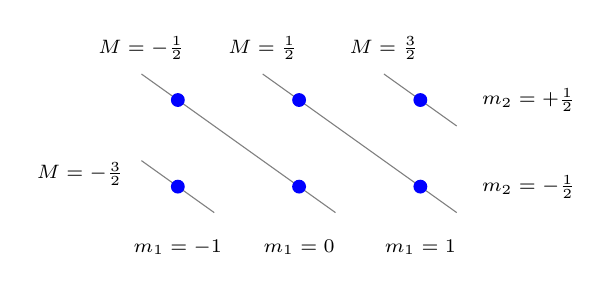
\begin{tikzpicture}[scale=1.1]
% diagonals of constant M = m1 + m2
\draw[thin, gray] (0.98,0.8) -- (1.82,0.2);
\draw[thin, gray] (-0.42,0.8) -- (1.82,-0.8);
\draw[thin, gray] (-1.82,0.8) -- (0.42,-0.8);
\draw[thin, gray] (-1.82,-0.2) -- (-0.98,-0.8);
% the six uncoupled states
\foreach \x in {-1,0,1} \foreach \y in {-0.5,0.5} {
  \fill[color=blue] (1.4*\x, \y) circle (0.08);
}
% M labels
\node[above] at (0.98,0.85) {\scriptsize $M = \tfrac32$};
\node[above] at (-0.42,0.85) {\scriptsize $M = \tfrac12$};
\node[above] at (-1.82,0.85) {\scriptsize $M = -\tfrac12$};
\node[left] at (-1.92,-0.35) {\scriptsize $M = -\tfrac32$};
% row and column labels
\node[right] at (2.0,0.5) {\scriptsize $m_2 = +\tfrac12$};
\node[right] at (2.0,-0.5) {\scriptsize $m_2 = -\tfrac12$};
\foreach \x/\l in {-1/{-1}, 0/{0}, 1/{1}} \node[below] at (1.4*\x,-1.0) {\scriptsize $m_1 = \l$};
\end{tikzpicture}
\end{center}

The picture makes the counting argument transparent: the multiplicities $d(M)$ along the diagonals are $1,2,2,1$ for $M = \frac32,\frac12,-\frac12,-\frac32$, so $n(\frac32) = 1$ and $n(\frac12) = 2-1 = 1$, giving $1 \otimes \frac12 = \frac32 \oplus \frac12$, of dimension $4+2 = 6$.

\subsection{Clebsch--Gordan Coefficients}

The two bases are related by a change of basis, whose matrix elements have a name.

\begin{definition}[Clebsch--Gordan Coefficients]
    Inserting the completeness relation for the uncoupled basis,
    $$
    \ket{J\,M} = \sum_{m_1,m_2}\ket{j_1\,m_1}\ket{j_2\,m_2}\,\braket{j_1\,m_1;\,j_2\,m_2}{J\,M},
    $$
    and the numbers $\braket{j_1 m_1; j_2m_2}{JM}$ are the \vocab{Clebsch--Gordan coefficients}.
\end{definition}

They vanish unless $M = m_1+m_2$ and $\abs{j_1-j_2}\leq J \leq j_1+j_2$; by convention they are taken real, so the transformation matrix is orthogonal and the inverse expansion uses the same numbers. In practice one computes them by the following recipe, which needs no tables:
\begin{enumerate}[label=(\roman*)]
    \item The state of maximal $M$ is unambiguous: $\ket{J{=}j_1{+}j_2,\,M{=}j_1{+}j_2} = \ket{j_1\,j_1}\ket{j_2\,j_2}$.
    \item Apply $J_- = J_-^{(1)} + J_-^{(2)}$ repeatedly to descend the top multiplet, using the known action of $J_-$ on each factor.
    \item The top state of the next multiplet, $\ket{J{=}j_1{+}j_2{-}1, M{=}J}$, is the (unique up to phase) normalised state with $M = j_1+j_2-1$ orthogonal to the one found in (ii). Then descend again, and repeat.
\end{enumerate}

\subsection{Two Spins: Singlet and Triplet}

Let us run the recipe on the most important case, $j_1 = j_2 = \frac12$. The theorem says
$$
\tfrac12 \otimes \tfrac12 = 1 \oplus 0,
$$
so the four-dimensional space splits into a three-dimensional $J=1$ multiplet and a one-dimensional $J=0$ multiplet. Explicitly, the top state is $\ket{1\,1} = \ket{\uparrow\uparrow}$, and applying $J_- = S_-^{(1)}+S_-^{(2)}$, using $S_-\ket\uparrow = \hbar\ket\downarrow$ and $S_-\ket\downarrow = 0$:
$$
J_-\ket{\uparrow\uparrow} = \hbar\left( \ket{\downarrow\uparrow} + \ket{\uparrow\downarrow} \right), \qquad \text{while} \qquad J_-\ket{1\,1} = \hbar\sqrt{2}\ket{1\,0},
$$
so $\ket{1\,0} = \frac{1}{\sqrt2}(\ket{\uparrow\downarrow}+\ket{\downarrow\uparrow})$; one more application gives $\ket{1\,{-1}} = \ket{\downarrow\downarrow}$. The remaining state is the normalised combination with $M = 0$ orthogonal to $\ket{1\,0}$.

\begin{proposition}[Singlet and Triplet]
    The $J=1$ \vocab{triplet} states are
    $$
    \ket{1\,1} = \ket{\uparrow\uparrow}, \qquad \ket{1\,0} = \tfrac{1}{\sqrt2}\left( \ket{\uparrow\downarrow}+\ket{\downarrow\uparrow} \right), \qquad \ket{1\,{-1}} = \ket{\downarrow\downarrow},
    $$
    and the $J = 0$ \vocab{singlet} state is
    $$
    \ket{0\,0} = \tfrac{1}{\sqrt2}\left( \ket{\uparrow\downarrow}-\ket{\downarrow\uparrow} \right).
    $$
    The triplet is symmetric under exchange of the two particles, the singlet antisymmetric.
\end{proposition}

\begin{center}
\begin{tikzpicture}[scale=1.0]
% uncoupled on the left
\node at (0,2.5) {\small uncoupled basis};
\foreach \y/\lab in {1.6/{\ket{\uparrow\uparrow}}, 1.05/{\ket{\uparrow\downarrow}}, 0.5/{\ket{\downarrow\uparrow}}, -0.05/{\ket{\downarrow\downarrow}}} {
  \draw[thick] (-0.7,\y) -- (0.7,\y);
  \node[left] at (-0.8,\y) {$\lab$};
}
\node at (0,-0.8) {\small $4$ states};
% arrow
\draw[->, very thick, color=gray] (1.6,0.8) -- (3.0,0.8);
\node[above, color=gray] at (2.3,0.85) {\small couple};
% coupled on the right
\node at (5.6,2.5) {\small coupled basis};
\foreach \y/\lab in {1.85/{\ket{1\,1}}, 1.3/{\ket{1\,0}}, 0.75/{\ket{1\,{-1}}}} {
  \draw[thick, color=blue] (4.4,\y) -- (5.9,\y);
  \node[right, color=blue] at (6.0,\y) {$\lab$};
}
\node[left, color=blue] at (4.3,1.3) {\small triplet};
\node[left, color=blue] at (4.3,0.95) {\small $J=1$};
\draw[thick, color=examplefg] (4.4,-0.15) -- (5.9,-0.15);
\node[right, color=examplefg] at (6.0,-0.15) {$\ket{0\,0}$};
\node[left, color=examplefg] at (4.3,-0.15) {\small singlet, $J=0$};
\node at (5.6,-0.8) {\small $3 + 1$ states};
\end{tikzpicture}
\end{center}

The names come from spectroscopy: in a magnetic field the $J=1$ states have distinct energies and produce three lines, while the $J=0$ state gives one. The energy splitting between the two families is already visible without a field, because
$$
\vv S^{(1)}\cdot \vv S^{(2)} = \frac{1}{2}\left( J^2 - (S^{(1)})^2 - (S^{(2)})^2 \right) = \frac{\hbar^2}{2}\left( J(J+1) - \frac34 - \frac34 \right)
= \begin{cases} +\frac{\hbar^2}{4} & \text{triplet},\\[2pt] -\frac{3\hbar^2}{4} & \text{singlet},\end{cases}
$$
so any interaction of the form $\lambda\, \vv S^{(1)}\cdot\vv S^{(2)}$ splits them. (This identity is the standard trick for evaluating dot products of angular momenta: rewrite them in terms of squares, which are diagonal in the coupled basis.) It is worth recording that the singlet is rotationally invariant -- being a $J=0$ state, it is annihilated by every $J_i$ and so looks the same along every axis. This innocuous fact is exactly what makes it the star of the EPR discussion.

\begin{example}[Spin--Orbit Coupling]
    An electron in an atomic orbital with $\ell = 1$ has $\vv J = \vv L + \vv S$ with $j_1 = 1$, $j_2 = \frac12$, so by the theorem $J = \frac32$ or $\frac12$: six states in all, splitting $4+2$. Relativistic effects generate a term
    $$
    H_{\mathrm{SO}} = \xi(r)\, \vv L \cdot \vv S = \frac{\xi(r)}{2}\left( J^2 - L^2 - S^2 \right),
    $$
    whose expectation value is $\frac{\hbar^2}{2}\expval{\xi}\left(j(j+1)-\ell(\ell+1)-\frac34\right)$, that is $+\frac{\hbar^2}{2}\expval\xi$ for $j = \frac32$ and $-\hbar^2\expval\xi$ for $j = \frac12$. This is the origin of the \emph{fine structure} doublet in the sodium spectrum (the famous yellow D lines), and shows why the coupled basis, not the uncoupled one, is the useful one whenever such a term is present.
\end{example}

\section{Transformations and Symmetries}\label{sec:symmetry}

We have already seen the key idea twice: time evolution is a one-parameter family of unitaries generated by the Hermitian operator $H$, and (in the Larmor example) rotation about the $z$-axis is generated by $S_z$. We now make this systematic. The pattern will be that every continuous symmetry of a quantum system is implemented by unitaries $U(\alpha) = \exp(-i\alpha Q/\hbar)$, that the generator $Q$ is an observable, and that $Q$ is conserved precisely when the symmetry is a symmetry of the Hamiltonian. This is Noether's theorem, and in quantum mechanics it is almost a triviality.

\subsection{Translations}

Consider translating a state of a particle in one dimension by $a$. In terms of wavefunctions this should send $\psi(x)$ to $\psi(x-a)$ -- a bump at the origin moves to a bump at $a$. Define $U(a)$ by
$$
\bra{x}U(a)\ket{\psi} = \psi(x - a).
$$
For infinitesimal $a$, Taylor expansion gives $\psi(x-a) = \psi(x) - a\psi'(x) + O(a^2)$, and since $-i\hbar\partial_x$ is the momentum operator,
$$
U(a) = I - \frac{i a P}{\hbar} + O(a^2).
$$
Composing $n$ translations by $a/n$ and letting $n \to \infty$ (or simply solving $\dd U/\dd a = -\frac{i}{\hbar}PU$),
$$
U(a) = \exp\left(-\frac{iaP}{\hbar}\right),
$$
and in three dimensions $U(\vv a) = \exp(-i\vv a \cdot \vv P/\hbar)$, which makes sense because the components of $\vv P$ commute with each other. So:

\begin{proposition}
    Momentum generates translations. The translation operators are unitary and form an abelian group, $U(\vv a) U(\vv b) = U(\vv a + \vv b)$.
\end{proposition}

It is worth checking the effect on operators. Since translating the state and translating the observable should be inverse operations,
$$
U(a)^\dagger X U(a) = X + a, \qquad U(a)^\dagger P U(a) = P,
$$
the first of which one can verify directly from $e^{B}Ae^{-B} = A + [B,A] + \frac{1}{2!}[B,[B,A]]+\cdots$ (the \emph{Baker--Campbell--Hausdorff} lemma, proved by differentiating $f(s) = e^{sB}Ae^{-sB}$) with $B = iaP/\hbar$: the series terminates after one term since $[P, X] = -i\hbar$ is a constant.

\begin{remark}
    The canonical commutation relation is thus \emph{equivalent} to the statement that $P$ generates translations of $X$. Read this way, $[X,P] = i\hbar$ stops looking like an arbitrary postulate.
\end{remark}

\subsection{Rotations}

The same logic applies to rotations, with two differences: the group is non-abelian, and the answer knows about spin. A rotation by angle $\theta$ about the axis $\vv n$ should be implemented by
$$
U(\theta, \vv n) = \exp\left( -\frac{i \theta \, \vv{n}\cdot\vv{J}}{\hbar} \right),
$$
where $\vv J$ is the total angular momentum. For a spinless particle we can check this directly: taking $\vv n = \vv e_3$ and using $L_z = -i\hbar\partial_\phi$,
$$
\exp\left( -\frac{i\theta L_z}{\hbar} \right) = \exp\left( -\theta \frac{\partial}{\partial \phi} \right),
$$
which is precisely the Taylor-series operator sending $\psi(r,\theta',\phi)$ to $\psi(r,\theta',\phi - \theta)$: a rotation. The failure of rotations about different axes to commute is encoded in $[J_i,J_j] = i\hbar\epsilon_{ijk}J_k$; indeed expanding both sides of $U(\alpha,\vv e_1)U(\beta, \vv e_2)U(\alpha,\vv e_1)^{-1}U(\beta,\vv e_2)^{-1}$ to second order reproduces exactly the commutator.

Under a rotation, a \vocab{vector operator} $\vv V$ -- one which transforms like $\vv X$ or $\vv P$ -- satisfies
$$
U^\dagger V_i U = R_{ij}V_j, \qquad \text{equivalently} \qquad [J_i, V_j] = i\hbar\epsilon_{ijk}V_k,
$$
where $R$ is the corresponding $3\times3$ rotation matrix. A \vocab{scalar operator} $S$ satisfies $[J_i, S] = 0$; examples are $r$, $P^2$, $L^2$ and $\vv L\cdot\vv S$.

\begin{remark}[Spin and the Double Cover]
    For spin-$\frac12$, $U(\theta, \vv n) = \exp(-\frac{i\theta}{2}\vv n \cdot \vv\sigma) = \cos\frac\theta2 I - i \sin\frac\theta2 \,\vv n\cdot\vv\sigma$, so
    $$
    U(2\pi, \vv n) = -I.
    $$
    A rotation by $2\pi$ -- which is no rotation at all -- acts as $-1$ on the state. This is consistent, because states are rays and an overall sign is unobservable; but it means the map from rotations to unitaries is only defined up to sign. What we really have is a representation of $SU(2)$, which is a double cover of $SO(3)$. Half-integer $j$ gives genuine $SU(2)$ representations that are not representations of $SO(3)$ -- another way of seeing why orbital angular momentum, which acts on honest functions on space, must have integer $\ell$. And the sign is not entirely unobservable: in an interference experiment where one arm rotates a neutron by $2\pi$ and the other does not, the relative sign is real and measurable, and has been measured.
\end{remark}

\subsection{Symmetries, Conservation and Degeneracy}

\begin{definition}[Symmetry]
    A unitary operator $U$ is a \vocab{symmetry} of a system with Hamiltonian $H$ if
    $$
    U^\dagger H U = H, \qquad \text{equivalently} \qquad [U, H] = 0.
    $$
\end{definition}

For a continuous family $U(\alpha) = e^{-i\alpha Q/\hbar}$, differentiating at $\alpha = 0$ shows this is equivalent to $[Q, H] = 0$. The consequences are immediate and important.

\begin{theorem}[Symmetry and Conservation]
    If $Q$ generates a symmetry of $H$ then $Q$ is a conserved quantity: $\expval{Q}$ and the whole probability distribution of $Q$ are constant in time.
\end{theorem}
\begin{proof}
    This is the corollary of \S2.2: $[Q,H] = 0$ and $Q$ has no explicit time dependence, so $\dd Q_H/\dd t = 0$.
\end{proof}

\begin{theorem}[Symmetry and Degeneracy]
    If $U$ is a symmetry and $\ket\psi$ is an energy eigenstate with $H\ket\psi = E\ket\psi$, then $U\ket\psi$ is also an energy eigenstate with the same $E$. Consequently, if the set $\{U\ket\psi\}$ over all symmetries $U$ spans a space of dimension $d > 1$, the level $E$ is at least $d$-fold degenerate.
\end{theorem}
\begin{proof}
    $H(U\ket\psi) = UH\ket\psi = E \, U\ket\psi$.
\end{proof}

This is the deepest structural fact in the subject, and answers a question left dangling in IB: \emph{why} do energy levels come with degeneracies? Because the eigenspaces of $H$ are invariant under the symmetry group, and therefore carry representations of it. For a rotationally invariant Hamiltonian, $[H, J_i] = 0$, so each energy eigenspace is a sum of angular momentum multiplets, and every level automatically has degeneracy $2j+1$ for some $j$: the $(2\ell+1)$-fold degeneracy of the hydrogen levels in $m$ is a theorem about $SO(3)$, not an accident of the Coulomb potential.

\begin{example}[Accidental Degeneracy]
    Hydrogen has a larger degeneracy than rotational symmetry demands: the level $E_n$ has degeneracy $n^2$, with all $\ell < n$ appearing, whereas rotational symmetry alone would allow the different $\ell$ to have different energies (as they do in every other atom). This is not an accident: the Coulomb problem has an extra conserved vector, the quantum \emph{Runge--Lenz vector}
    $$
    \vv A = \frac{1}{2m}\left( \vv P \times \vv L - \vv L \times \vv P \right) - \frac{e^2}{4\pi\epsilon_0}\frac{\vv X}{r},
    $$
    which commutes with $H$ and enlarges the symmetry from $SO(3)$ to $SO(4)$. The whole hydrogen spectrum can be derived from this algebra without solving a differential equation, exactly as we did for the oscillator. The three-dimensional isotropic oscillator has a similar story with symmetry group $SU(3)$.
\end{example}

\subsection{Parity}

Not all symmetries are continuous. The most important discrete one is spatial inversion.

\begin{definition}[Parity]
    The \vocab{parity operator} $\Pi$ acts on wavefunctions by $(\Pi\psi)(\vv x) = \psi(-\vv x)$.
\end{definition}

\begin{proposition}
    $\Pi$ is Hermitian and unitary with $\Pi^2 = I$, so its eigenvalues are $\pm1$. Moreover
    $$
    \Pi \vv X \Pi = -\vv X, \qquad \Pi \vv P \Pi = -\vv P, \qquad \Pi \vv L \Pi = +\vv L, \qquad \Pi\vv S\Pi = +\vv S.
    $$
\end{proposition}
\begin{proof}
    Hermiticity is a change of variables in the integral $\int \phi^*(\vv x)\psi(-\vv x)\dd^3x$, and $\Pi^2 = I$ is clear; together these give unitarity. The action on $\vv X$ and $\vv P$ follows from $\Pi\psi(\vv x) = \psi(-\vv x)$ and the chain rule, and then $\vv L = \vv X \times \vv P$ picks up two signs, so is unchanged. Spin, being an angular momentum, transforms the same way as $\vv L$.
\end{proof}

Quantities like $\vv L$ and $\vv S$ that are \emph{even} under parity are called \vocab{axial} (or pseudo-) vectors, while $\vv X, \vv P$ are \vocab{polar} vectors -- the same distinction as in classical mechanics. Since $\Pi$ commutes with $L^2$ and $\vv L$, it acts as a constant on each multiplet, and one finds that constant by evaluating on $Y_{\ell\ell}\propto \sin^\ell\theta\, e^{i\ell\phi}$: inversion sends $(\theta,\phi)\mapsto(\pi-\theta,\phi+\pi)$, which multiplies this by $(-1)^\ell$. So
$$
\Pi \, Y_{\ell m} = (-1)^\ell \, Y_{\ell m}.
$$

If $[\Pi, H] = 0$ -- which holds whenever the potential is even, $U(-\vv x) = U(\vv x)$ -- then parity is conserved and we may choose energy eigenstates of definite parity. The most useful consequence is a \emph{selection rule}.

\begin{proposition}[Parity Selection Rule]
    Let $\ket\psi$ and $\ket\phi$ have definite parities $\eta_\psi, \eta_\phi = \pm1$, and let $V$ be an operator with $\Pi V \Pi = \eta_V V$. Then
    $$
    \mel{\phi}{V}{\psi} = 0 \qquad \text{unless} \qquad \eta_\phi\, \eta_V\, \eta_\psi = +1.
    $$
\end{proposition}
\begin{proof}
    Insert $\Pi^2 = I$ twice: $\mel{\phi}{V}{\psi} = \mel{\phi}{\Pi \Pi V \Pi \Pi}{\psi} = \eta_\phi \eta_V \eta_\psi \mel{\phi}{V}{\psi}$.
\end{proof}

For instance $\vv X$ is parity-odd, so $\mel{\phi}{\vv X}{\psi}$ vanishes between states of the same parity. Since the leading interaction of an atom with light is the electric dipole term $\propto \vv E \cdot \vv X$, this is exactly the rule that atomic transitions must change parity -- so, using $\Pi Y_{\ell m} = (-1)^\ell Y_{\ell m}$, they must change $\ell$ by an odd number, and a more refined argument using rotational symmetry sharpens this to $\Delta \ell = \pm1$. Selection rules of this kind are why atomic spectra contain far fewer lines than the number of pairs of levels would suggest.

\begin{remark}[Time Reversal]
    The other classic discrete symmetry is time reversal, which should send $\vv X \mapsto \vv X$ and $\vv P \mapsto -\vv P$ (and $\vv J \mapsto -\vv J$). No unitary can do this: it would preserve $[X,P] = i\hbar$ while flipping the sign of the right-hand side. The resolution, due to Wigner, is that time reversal is implemented by an \emph{antiunitary} operator $\Theta$ -- one that is antilinear, $\Theta(\lambda\ket\psi) = \lambda^*\Theta\ket\psi$, and satisfies $\braket{\Theta\phi}{\Theta\psi} = \braket{\phi}{\psi}^*$. For a spinless particle $\Theta$ is simply complex conjugation of the wavefunction, and indeed if $\psi(\vv x, t)$ solves the Schr\"odinger equation with real potential then so does $\psi^*(\vv x, -t)$. Because $\Theta$ is not linear it has no eigenvalues in the usual sense and generates no conservation law; its main structural consequence is \emph{Kramers' degeneracy}, that a time-reversal-invariant system with half-integer total angular momentum has all its energy levels degenerate to even order.
\end{remark}

\section{Time-Independent Perturbation Theory}\label{sec:pt}

The list of quantum systems we can solve exactly is embarrassingly short: the free particle, the square well, the oscillator, the hydrogen atom, and a handful of others. Almost every real problem is one of these with something extra added -- an electric field, a magnetic field, a second electron, a slight anharmonicity. Perturbation theory is the systematic way of getting approximate answers by treating the extra piece as small.

The setup throughout is
$$
H = H_0 + \lambda V,
$$
where the \vocab{unperturbed} Hamiltonian $H_0$ is solved,
$$
H_0 \ket{n^{(0)}} = E_n^{(0)}\ket{n^{(0)}},
$$
with $\{\ket{n^{(0)}}\}$ a complete orthonormal set, and $\lambda$ is a small dimensionless parameter that we use to organise the expansion (and often set to $1$ at the end). We write $V_{mn} = \mel{m^{(0)}}{V}{n^{(0)}}$.

\subsection{The Non-Degenerate Case}

Assume first that the level $E_n^{(0)}$ we are interested in is non-degenerate, and posit power series
$$
E_n = E_n^{(0)} + \lambda E_n^{(1)} + \lambda^2 E_n^{(2)} + \cdots, \qquad
\ket{n} = \ket{n^{(0)}} + \lambda \ket{n^{(1)}} + \lambda^2\ket{n^{(2)}} + \cdots.
$$
We may normalise the expansion by choosing $\braket{n^{(0)}}{n^{(k)}} = 0$ for $k\geq1$ -- the component of the correction along the original state is pure rescaling, and can be removed at the end. Substituting into $H\ket n = E_n \ket n$ and collecting powers of $\lambda$:
\begin{align*}
    \lambda^0: & \quad \left( H_0 - E_n^{(0)} \right)\ket{n^{(0)}} = 0, \\
    \lambda^1: & \quad \left( H_0 - E_n^{(0)} \right)\ket{n^{(1)}} = \left( E_n^{(1)} - V \right)\ket{n^{(0)}}, \\
    \lambda^2: & \quad \left( H_0 - E_n^{(0)} \right)\ket{n^{(2)}} = \left( E_n^{(1)} - V \right)\ket{n^{(1)}} + E_n^{(2)}\ket{n^{(0)}}.
\end{align*}
Now project each equation onto the unperturbed basis. Taking $\bra{n^{(0)}}$ of the $\lambda^1$ equation, the left-hand side vanishes (as $H_0$ is Hermitian and acts leftwards as $E_n^{(0)}$), giving at once
$$
\boxed{\;E_n^{(1)} = V_{nn} = \mel{n^{(0)}}{V}{n^{(0)}}.\;}
$$
Taking $\bra{m^{(0)}}$ with $m \neq n$ gives $(E_m^{(0)} - E_n^{(0)})\braket{m^{(0)}}{n^{(1)}} = -V_{mn}$, so
$$
\ket{n^{(1)}} = \sum_{m\neq n}\frac{V_{mn}}{E_n^{(0)} - E_m^{(0)}}\ket{m^{(0)}}.
$$
Finally, taking $\bra{n^{(0)}}$ of the $\lambda^2$ equation and using $\braket{n^{(0)}}{n^{(1)}} = 0$,
$$
0 = -\mel{n^{(0)}}{V}{n^{(1)}} + E_n^{(2)}, \qquad \text{so} \qquad
\boxed{\;E_n^{(2)} = \sum_{m\neq n}\frac{\abs{V_{mn}}^2}{E_n^{(0)} - E_m^{(0)}}.\;}
$$

\begin{theorem}[Rayleigh--Schr\"odinger Perturbation Theory]
    To second order, and setting $\lambda = 1$,
    $$
    E_n = E_n^{(0)} + V_{nn} + \sum_{m \neq n} \frac{\abs{V_{mn}}^2}{E_n^{(0)}-E_m^{(0)}} + O(V^3),
    $$
    with corresponding state $\ket n = \ket{n^{(0)}} + \sum_{m\neq n}\frac{V_{mn}}{E_n^{(0)}-E_m^{(0)}}\ket{m^{(0)}} + O(V^2)$.
\end{theorem}

Several things are worth noticing. The first-order shift is just the expectation value of the perturbation in the unperturbed state -- entirely intuitive. The second-order shift for the \emph{ground state} is always negative, since every denominator $E_0^{(0)}-E_m^{(0)}$ is negative: mixing in other states can only push the ground state down. More generally levels `repel': a pair of levels contributes to each other's shift with opposite signs, pushing the higher one up and the lower one down. And the whole thing is an asymptotic expansion in $V/\Delta E$, where $\Delta E$ is the typical level spacing; it fails badly if any denominator is small, which is exactly the situation of degeneracy.

\begin{center}
\begin{tikzpicture}[scale=1.0]
% guide lines at the unperturbed heights
\foreach \y in {0, 1.6, 2.9} \draw[dashed, gray, thin] (0,\y) -- (6.2,\y);
% unperturbed levels
\foreach \y/\lab in {0/{E_0^{(0)}}, 1.6/{E_1^{(0)}}, 2.9/{E_2^{(0)}}} {
  \draw[very thick] (0,\y) -- (2.0,\y);
  \node[left] at (-0.1,\y) {$\lab$};
}
\node at (1.0,-1.35) {\small $H_0$};
% perturbed levels
\foreach \y/\lab in {-0.6/{E_0}, 1.9/{E_1}, 2.6/{E_2}} {
  \draw[very thick, color=blue] (4.2,\y) -- (6.2,\y);
  \node[right, color=blue] at (6.3,\y) {$\lab$};
}
\node at (5.2,-1.35) {\small $H = H_0 + V$};
% shift arrows
\draw[<->, color=examplefg] (3.1,0.0) -- (3.1,-0.6);
\node[left, color=examplefg] at (3.0,-0.3) {\small $\delta E_0$};
\draw[<->, color=examplefg] (3.1,1.6) -- (3.1,1.9);
\draw[<->, color=examplefg] (3.1,2.9) -- (3.1,2.6);
\end{tikzpicture}
\end{center}

\begin{example}[The Anharmonic Oscillator]
    Take $H = \frac{P^2}{2m} + \frac12 m\omega^2X^2 + \lambda X^4$. The first-order shift of the level $n$ is $\lambda\mel{n}{X^4}{n}$, which is easy with creation and annihilation operators. Writing $X = \alpha(a+a^\dagger)$ with $\alpha = \sqrt{\hbar/2m\omega}$, we need the terms of $(a+a^\dagger)^4$ with equal numbers of $a$ and $a^\dagger$; keeping track of the orderings,
    $$
    \mel{n}{X^4}{n} = \alpha^4\left( 3 + 6n + 6n^2 \right) = 3\left(\frac{\hbar}{2m\omega}\right)^2\left( 2n^2+2n+1 \right).
    $$
    (A quick check: for $n=0$ this is $3\alpha^4 = 3\expval{X^2}_0^2$, as it should be for a Gaussian.) So
    $$
    E_n \approx \left( n + \frac12 \right)\hbar\omega + \frac{3\lambda\hbar^2}{4m^2\omega^2}\left(2n^2+2n+1\right).
    $$
    The correction grows like $n^2$, so the expansion is only good for $n \ll m^2\omega^3/\lambda\hbar$: perturbation theory in a fixed $\lambda$ eventually fails for high levels, which is physically obvious since a highly excited state explores large $x$ where $\lambda x^4$ dominates $\frac12 m\omega^2x^2$.
\end{example}

\begin{example}[A Two-State System, Exactly and Perturbatively]
    Let $H = \begin{pmatrix} E_1 & v \\ v & E_2\end{pmatrix}$ with $E_1 < E_2$ and $v$ real. The exact eigenvalues are
    $$
    E_\pm = \frac{E_1+E_2}{2} \pm \sqrt{ \left(\frac{E_2-E_1}{2}\right)^2 + v^2 },
    $$
    and expanding the square root for $v \ll E_2 - E_1$ gives
    $$
    E_- = E_1 - \frac{v^2}{E_2 - E_1} + O(v^4), \qquad E_+ = E_2 + \frac{v^2}{E_2-E_1}+O(v^4),
    $$
    exactly matching the second-order formula (the first-order shifts vanish since the diagonal of $V$ is zero). Note the level repulsion, and note also what happens as $E_2 \to E_1$: the perturbative answer diverges but the exact one does not -- it becomes $E_\pm = E_1 \pm v$, a splitting \emph{linear} in $v$. This is the degenerate case, and it needs different treatment.
\end{example}

\subsection{The Degenerate Case}

Suppose now that $E^{(0)}$ is an eigenvalue of $H_0$ with a $d$-dimensional eigenspace $\mathcal{H}_0$, spanned by orthonormal $\ket{1},\dots,\ket{d}$. The non-degenerate formulae break down because of the vanishing denominators; but the two-state example above shows what is really going on. \emph{Any} basis of $\mathcal{H}_0$ diagonalises $H_0$, so at zeroth order we do not know which states to expand around, and we must let the perturbation tell us.

Write the true eigenstate as $\ket\psi = \ket{\psi^{(0)}} + \lambda\ket{\psi^{(1)}}+\cdots$ with $\ket{\psi^{(0)}} = \sum_{i=1}^d c_i \ket{i} \in \mathcal{H}_0$ unknown. The order-$\lambda$ equation is as before,
$$
\left( H_0 - E^{(0)} \right)\ket{\psi^{(1)}} = \left( E^{(1)} - V \right)\ket{\psi^{(0)}},
$$
and projecting onto $\bra{j}$ for $j = 1,\dots,d$ kills the left-hand side, leaving
$$
\sum_{i}\mel{j}{V}{i}\, c_i = E^{(1)} c_j.
$$

\begin{theorem}[Degenerate Perturbation Theory]
    The first-order energy shifts of a degenerate level are the eigenvalues of the $d\times d$ Hermitian matrix
    $$
    \mathcal{V}_{ji} = \mel{j}{V}{i}, \qquad i,j = 1,\dots,d,
    $$
    and the correct zeroth-order states are the corresponding eigenvectors.
\end{theorem}

So the recipe is: restrict the perturbation to the degenerate subspace and diagonalise it. If the eigenvalues of $\mathcal{V}$ are distinct, the degeneracy is completely lifted at first order and one may then continue with non-degenerate perturbation theory in the new basis. If some remain equal, the degeneracy survives to first order and one must go further -- often it is protected by a symmetry that $V$ does not break, in which case it survives to all orders.

\begin{center}
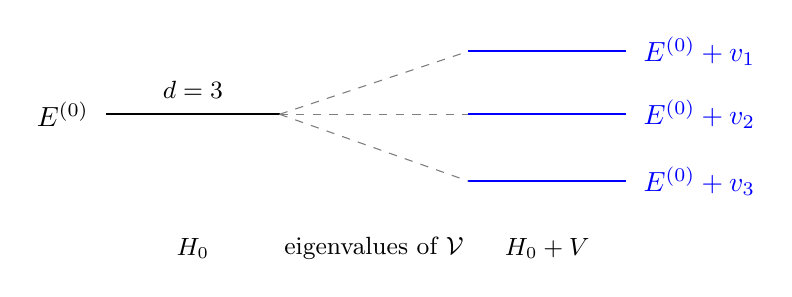
\begin{tikzpicture}[scale=1.0]
% degenerate level
\draw[thick] (0,1.2) -- (2.2,1.2);
\node[left] at (-0.1,1.2) {$E^{(0)}$};
\node[above] at (1.1,1.28) {\small $d = 3$};
% split levels
\foreach \y/\lab in {2.0/{E^{(0)}+v_1}, 1.2/{E^{(0)}+v_2}, 0.35/{E^{(0)}+v_3}} {
  \draw[thick, color=blue] (4.6,\y) -- (6.6,\y);
  \draw[dashed, gray] (2.2,1.2) -- (4.6,\y);
  \node[right, color=blue] at (6.7,\y) {$\lab$};
}
\node at (1.1,-0.5) {\small $H_0$};
\node at (5.6,-0.5) {\small $H_0 + V$};
\node at (3.4,-0.5) {\small eigenvalues of $\mathcal{V}$};
\end{tikzpicture}
\end{center}

\begin{example}[The Normal Zeeman Effect]
    Put a hydrogen atom in a uniform magnetic field $\vv B = B \vv e_3$. The orbital motion of the electron gives a magnetic moment $\vv\mu = -\frac{e}{2m_e}\vv L$, so (ignoring spin for the moment)
    $$
    V = -\vv\mu\cdot\vv B = \frac{eB}{2m_e}L_z = \frac{\mu_B B}{\hbar}L_z,
    $$
    where $\mu_B = e\hbar/2m_e$ is the \vocab{Bohr magneton}. The unperturbed level $E_n$ is $n^2$-fold degenerate, so we should diagonalise $V$ on that subspace -- but it is already diagonal in the basis $\ket{n\,\ell\,m}$, with eigenvalues $\mu_B B m$. Hence
    $$
    E_{n\ell m} = E_n + \mu_B B\, m, \qquad m = -\ell,\dots,\ell,
    $$
    and each $\ell$-multiplet splits into $2\ell+1$ equally spaced levels. This is exactly the degeneracy-versus-symmetry story of \S\ref{sec:symmetry} run in reverse: the field picks out an axis, breaking $SO(3)$ down to rotations about $\vv e_3$, and the degeneracy protected by the larger group is destroyed.
\end{example}

\begin{remark}[The Anomalous Zeeman Effect]
    Including spin, the moment is $\vv \mu = -\frac{e}{2m_e}(\vv L + 2\vv S)$ -- the factor of $2$ being the electron's $g$-factor, a prediction of the Dirac equation -- so
    $$
    V = \frac{\mu_B B}{\hbar}\left( L_z + 2S_z \right) = \frac{\mu_B B}{\hbar}\left( J_z + S_z \right).
    $$
    If the field is weak compared with the spin--orbit coupling, one must work in the coupled basis $\ket{j\,m_j}$, where $S_z$ is not diagonal but its restriction to fixed $j$ turns out to be proportional to $J_z$; the shift is $\mu_B B g_J m_j$ with the \vocab{Land\'e $g$-factor}
    $$
    g_J = 1 + \frac{j(j+1)+s(s+1)-\ell(\ell+1)}{2j(j+1)}.
    $$
    In a strong field the spin--orbit term is instead the perturbation, and one works in the uncoupled basis; the two regimes give different-looking spectra, and the crossover between them (the Paschen--Back effect) is a nice illustration of why choosing the right zeroth-order basis is the whole art of degenerate perturbation theory.
\end{remark}

\begin{example}[The Linear Stark Effect]
    Put hydrogen in a uniform electric field $\vv{\mathcal{E}} = \mathcal{E}\vv{e}_3$, so $V = e\mathcal{E}Z$. For the ground state $\ket{1\,0\,0}$, the first-order shift vanishes by parity ($Z$ is odd, $\ket{100}$ has definite parity), so the effect is quadratic in $\mathcal{E}$ -- the atom has no permanent dipole moment.

    The $n=2$ level is different. It is four-fold degenerate (ignoring spin), spanned by $\ket{200}, \ket{210},\ket{21{\pm}1}$, and we must diagonalise the $4\times4$ matrix of $V$. Almost all entries vanish: $\mel{2\ell m}{Z}{2\ell'm'} = 0$ unless $m = m'$ (since $Z$ commutes with $L_z$) and unless $\ell,\ell'$ have opposite parity (since $Z$ is parity-odd). The only surviving matrix element is between $\ket{200}$ and $\ket{210}$, and an explicit integral gives $\mel{200}{Z}{210} = -3a_0$ with $a_0$ the Bohr radius. So in the basis $(\ket{200},\ket{210},\ket{211},\ket{21{-}1})$,
    $$
    \mathcal{V} = -3ea_0\mathcal{E}\begin{pmatrix}0&1&0&0\\1&0&0&0\\0&0&0&0\\0&0&0&0\end{pmatrix},
    $$
    with eigenvalues $\mp3ea_0\mathcal{E}$ and $0$ (twice). The level splits into three, with the outer two shifting \emph{linearly} in the field -- so an excited hydrogen atom does behave as though it has a permanent dipole moment of size $3ea_0$. The reason it can is precisely the accidental degeneracy between the $2s$ and $2p$ states, which lets the field mix states of opposite parity at no energy cost.
\end{example}

\subsection{The Variational Principle}

Perturbation theory needs a nearby solvable problem. When there is none, the following gives a completely different handle, and in particular a rigorous \emph{bound}.

\begin{theorem}[Variational Principle]
    Let $H$ have ground state energy $E_0$. Then for every normalised $\ket\psi \in \mathcal{H}$,
    $$
    \mel{\psi}{H}{\psi} \geq E_0,
    $$
    with equality if and only if $\ket\psi$ is a ground state.
\end{theorem}
\begin{proof}
    Expand in an orthonormal basis of eigenstates, $\ket\psi = \sum_n a_n \ket n$ with $\sum_n \abs{a_n}^2 = 1$. Then
    $$
    \mel{\psi}{H}{\psi} = \sum_n E_n \abs{a_n}^2 \geq E_0 \sum_n \abs{a_n}^2 = E_0,
    $$
    with equality iff $a_n = 0$ whenever $E_n > E_0$.
\end{proof}

The proof is trivial; the power comes from what one does with it. Choose a family of \vocab{trial states} $\ket{\psi_\alpha}$ depending on parameters $\alpha$, compute
$$
\mathcal{E}(\alpha) = \frac{\mel{\psi_\alpha}{H}{\psi_\alpha}}{\braket{\psi_\alpha}{\psi_\alpha}},
$$
and minimise over $\alpha$. Whatever family we pick, the result is a genuine upper bound on $E_0$, and if the family happens to contain a good approximation to the true ground state the bound will be tight. Even a crude family usually does well, because $\mathcal{E}$ is \emph{stationary} at the true ground state: an error of size $\epsilon$ in the state produces an error of size $\epsilon^2$ in the energy.

\begin{center}
\begin{tikzpicture}[scale=1.0]
\draw[->] (-0.3,0) -- (5.6,0) node[right] {\small $\alpha$};
\draw[->] (0,-0.3) -- (0,3.3) node[above] {\small $\mathcal{E}(\alpha)$};
% true ground state energy
\draw[thick, color=examplefg] (0,0.7) -- (5.3,0.7);
\node[right, color=examplefg] at (5.35,0.7) {\small $E_0$};
% trial curve, minimum above E_0
\draw[thick, color=blue, samples=120, smooth, domain=0.35:5.2] plot (\x, {1.15 + 1.35*(\x-2.6)*(\x-2.6)/4.2});
\draw[dashed, gray] (0,1.15) -- (2.6,1.15);
\draw[dashed, gray] (2.6,0) -- (2.6,1.15);
\fill[color=blue] (2.6,1.15) circle (0.07);
\node[below] at (2.6,-0.05) {\small $\alpha_*$};
\node[left] at (-0.05,1.15) {\small $\mathcal{E}(\alpha_*)$};
\draw[<->, color=examplefg] (3.9,0.72) -- (3.9,1.13);
\node[right, color=examplefg] at (3.95,0.93) {\scriptsize error};
\end{tikzpicture}
\end{center}

\begin{example}[The Quartic Oscillator]
    Take $H = \frac{P^2}{2m} + \lambda X^4$, which has no exact solution and no small parameter to perturb in (there is no quadratic term at all). Use the Gaussian family
    $$
    \psi_a(x) = \left(\frac{a}{\pi}\right)^{1/4}e^{-ax^2/2},
    $$
    for which $\expval{X^2} = \frac{1}{2a}$, $\expval{X^4} = 3\expval{X^2}^2 = \frac{3}{4a^2}$ and $\expval{P^2} = \frac{\hbar^2 a}{2}$. Hence
    $$
    \mathcal{E}(a) = \frac{\hbar^2 a}{4m} + \frac{3\lambda}{4a^2}.
    $$
    Setting $\mathcal{E}'(a) = 0$ gives $a_*^3 = 6m\lambda/\hbar^2$, and substituting back,
    $$
    E_0 \leq \mathcal{E}(a_*) \approx 0.681 \left( \frac{\hbar^2}{m} \right)^{2/3}\lambda^{1/3}.
    $$
    Note first that the $\lambda^{1/3}$ scaling is exact -- it follows from dimensional analysis, since $\hbar^2/m$ and $\lambda$ can be combined into an energy in only one way. Numerical solution of the Schr\"odinger equation gives the true coefficient as $0.668$, so our one-parameter guess is within $2\%$.
\end{example}

\begin{remark}[Excited States]
    The principle extends: if $\ket{\psi}$ is orthogonal to the exact ground state, then $\expval{H}_\psi \geq E_1$, and so on up the spectrum. In practice we rarely know the exact ground state, but symmetry often does the job for free -- any odd trial function is automatically orthogonal to an even ground state, so minimising over odd trial functions bounds the first excited state of a symmetric potential.
\end{remark}

\begin{remark}
    A pleasant corollary: \emph{any} attractive potential well in one dimension, however shallow, has at least one bound state. Take a trial Gaussian of width $\sigma$; the kinetic energy costs $O(\hbar^2/m\sigma^2)$ while the potential energy gains $O(-\int U/\sigma)$ for large $\sigma$, and the latter wins as $\sigma\to\infty$, giving $\mathcal{E} < 0$ for some trial state and hence a bound state. The same argument fails in three dimensions, where the kinetic cost scales the same way but the potential gain is weaker -- and indeed shallow three-dimensional wells have no bound states.
\end{remark}

\end{document}
